% FILE: main.tex  Version 2.1
% AUTHOR:
% Universit�t Duisburg-Essen, Standort Duisburg
% AG Prof. Dr. G�nter T�rner
% Verena Gondek, Andy Braune, Henning Kerstan
% Fachbereich Mathematik
% Lotharstr. 65., 47057 Duisburg
% entstanden im Rahmen des DFG-Projektes DissOnlineTutor
% in Zusammenarbeit mit der
% Humboldt-Universitaet zu Berlin
% AG Elektronisches Publizieren
% Joanna Rycko
% und der
% DNB - Deutsche Nationalbibliothek

\chapter{Discourse-Aware Sentiment Analysis}

Although coarse-grained sentiment analysis methods presented in the
previous chapter do a fairly good job at classifying the overall
polarity of a message,
%% putting their best leg forward to incorporate the compositional
%% principle into that prediction,
a crucial limitation of all these systems is that they completely
overlook the structural nature of their input by either considering it
as a single whole (\eg{} bag-of-features approaches) or analyzing it
as a monotone sequence of equally important elements (\eg{} recurrent
neural methods).  Unfortunately, both of these solutions violate the
hierarchical principle of language \cite{Saussure:90,Hjelmslev:70},
which states that complex linguistic units are formed from smaller
language elements in the bottom-up way: \eg{} words are created by
putting together morphemes, sentences are made of several words, and
discourse is composed of multiple coherent sentences.  Moreover, apart
from this inherent structural heterogeneity, even units of the same
linguistic level often play a different role and are of unequal
importance when joined syntagmatically into the higher-level whole:
for example, in words, the root morpheme typically conveys more
lexical information than the affixes; in sentences, the syntactic head
usually dominates its grammatic dependents; and, in discourse, one of
the sentences frequently expresses more prominent ideas than the rest
of the text.
%% At the same time, even auxiliary modifying elements might completely
%% overturn the meaning of the central part to its opposite (cf. \emph{to
%%   like} vs. \emph{to dislike}; \emph{She enjoyed this song}
%% vs. \emph{She didn't enjoy this song}; \emph{Trump is a good
%%   businessman} vs. \emph{Trump is a good businessman, but a terrible
%%   employer}).

Exactly the lack of discourse information was one of the main reasons
for the misclassifications made by the systems of \citet{Severyn:15},
\citet{Baziotis:17}, and our own LBA method in Examples
\ref{snt:cgsa:exmp:severyn-error}, \ref{snt:cgsa:exmp:baziotis-error},
and \ref{snt:cgsa:exmp:lba-error}.  Since none of these approaches
explicitly took the discourse structure into account, we decided to
check whether making the last of these solutions (the LBA classifier)
aware of discourse phenomena would improve its results.  But before we
proceed to our experiments, we first would like to make a short
digression into the theory of discourse and give an overview of the
most popular approaches to text-level analysis that exist in the
literature nowadays.  Afterwards, in Section~\ref{sec:dasa:data}, we
will describe the way how we inferred discourse information for the
PotTS and SB10k data.  Then, in Section~\ref{sec:dasa:methods}, we
will summarize the current state of the art in discourse-aware
sentiment analysis (DASA) and also present our own methods, evaluating
them on the aforementioned corpora.  After analyzing the effects of
various common factors (such as the impact of the underlying sentiment
classifier and the amenability of various discourse relation subsets
to different DASA approaches), we will recap our results and summarize
our findings in the last part of this chapter.

\section{Discourse Analysis}\label{sec:dasa:theory}

Since the main focus of our experiments will be on \emph{discourse
  analysis}, we first need to clarify what discourse analysis actually
means and which common ways there are to represent and analyze
discourse automatically.

In a nutshell, discourse analysis is an area of research which
explores and analyzes language phenomena beyond the sentence level
\cite{Stede:11}.  Although the scope of this research can be quite
large, ranging from the use of pronouns in a sentence to the logical
composition of entire document, in our work we will primarily
concentrate on the coherence structure of the text, \ie{} its
segmentation into \emph{elementary discourse units} (typically single
propositions) and induction of hierarchical \emph{coherence relations}
(semantic or pragmatic links) between these EDUs.

Although the idea of splitting the text into smaller meaningful pieces
and inferring semantic relationships between these parts is anything
but new, dating back to the very origins of general linguistics
\cite{Aristotle:10} and in particular its structuralism branch
\cite{Saussure:90}, an especially big surge of interest in this field
happened in the 1970-s with the fundamental works of
\citet{vanDijk:72} and \citet{vanDijk:83}, who introduced the notion
of local and global coherence, defining the former as a set of ``rules
and conditions for the well-formed concatenation of pairs of sentences
in a linearly ordered sequence'' and specifying the latter as
contraints on the macro-structure of the narrative
\cite[see][]{Hoey:83}.  Similar ideas were also proposed
by~\citet{Longacre:79,Longacre:96}, who considered the paragraph as a
unit of tagmemic grammar which was composed of multiple sentences
according to a predefined set of compositional principles.  Almost
contemporarily with these works, \citet{Winter:77} presented an
extensive study of various lexical means that could connect two
sentences and grouped these means into two major categories:
\textsc{Matching} and \textsc{Logical Sequence}; depending on whether
they introduced sentences which were giving more details on the
preceding content or adding new information to the narrative.

The increased interest of traditional linguistics in text-level
analysis has rapidly spurred the attention of the broader NLP
community.  Among the first who stressed the importance of discourse
phenomena for automatic generation and understanding of texts was
\citet{Hobbs:79}, who argued that semantic links between sentences
were one the most important component for building a coherent
discourse.  Similarly to \citeauthor{Winter:77}, \citeauthor{Hobbs:79}
also proposed a classification of inter-sentence relations, dividing
them into \textsc{Elaboration}, \textsc{Parallel}, and
\textsc{Contrast}.  Albeit this taxonomy was obviously too small to
accommodate all possible semantic and pragmatic relationships that
could exist between any two clauses, this division had laid the
foundations for many successful approaches to automatic discourse
analysis that appeared in the following decades.

\textbf{RST.}\quad{}One of the best-known such
approaches---\emph{Rhetorical Structure Theory} or \emph{RST}---was
presented by~\citet{Mann:88}.  Besides revising \citeauthor{Hobbs:79}'
inventory of discourse relations and expanding it to 23 elements
(including new items such as \textsc{Antithesis},
\textsc{Circumstance}, \textsc{Evidence}, and \textsc{Elaboration}),
the authors also grouped all coherence links into nucleus-satellite
(hypotactic) and multinuclear (paratactic) ones, depending on whether
the arguments of these edges were of different or equal importance to
the content of the whole text.  Based on this grouping, they formally
described each relation as a set of constraints on the \emph{Nucleus}
(N), \emph{Satellite} (S), \emph{the N+S combination}, and \emph{the
  effect} of the whole combination on the reader (R).  An excerpt from
the original description of the \textsc{Antithesis} relation is given
in Example~\ref{dasa:exmp:rst-evidence}

\begin{example}[Definition of the \textsc{Antithesis} Relation]\label{dasa:exmp:rst-evidence}
  \textbf{Relation Name:} \textsc{Antithesis}

  \textbf{Constraints on N:} W has positive regard for the situation
  presented in N

  \textbf{Constraints on S:} None

  \textbf{Constraints on the N+S Combination:} the situations presented
  in N and S are in contrast (\ie{} are
  \begin{inparaenum}[(a)]
  \item comprehended as the same in many respects,
  \item comprehended as differing in a few respects and
  \item compared with respect to one or more of these differences
  \end{inparaenum}
  ); because of an incompatibility that arises from the contrast, one
  cannot have positive regard for both the situations presented in N and
  S; comprehending S and the incompatibility between the situations
  presented in N and S increases R's positive regard for the situation
  presented in N

  \textbf{Effect:} R's positive regard for N is increased

  \textbf{Locus of the Effect:} N
\end{example}
The authors then defined the general structure of the discourse as a
projective (constituency) tree whose nodes were either elementary
discourse units or subtrees that were connected to each other via
these predefined coherence links.

You can see an example of such hierarchical coherence tree from the
original Rhetorical Structure Treebank \cite{Carlson:01a} in
Figure~\ref{dasa:fig:rst-tree}.

\begin{figure*}[htb!]\label{dasa:fig:rst-tree}
    {
    \small
    \centering
  \dirrel{}{
    \dirrel{Attribution}
           {\rstsegment{\refr{1}}}
           {}
           {\rstsegment{\refr{2}}}}
         {Interpretation-S}
         {\dirrel{Antithesis}
           {\rstsegment{\refr{3}}}
           {}
           {
             \dirrel{Attribution}
                    {\rstsegment{\refr{4}}}
                    {}
                    {
                      \dirrel{}
                             {
                               \dirrel{}{\rstsegment{\refr{5}}}{Comparison}{\rstsegment{\refr{6}}}
                             }
                             {Condition}
                             {\rstsegment{\refr{7}}}
                    }
           }
         }

         \begin{flushleft}
           \begin{rhetoricaltext}
             \unit[1]{Analysts said,}
             \unit[2]{profit for the dozen or so big drug makers, as a group, is estimated to have climbed between 11\% and 14\%.}
             \unit[3]{While that's not spectacular,}
             \unit[4]{Neil Sweig, an analyst with Prudential Bache, said}
             \unit[5]{that the rate of growth will ``look especially good}
             \unit[6]{as compared to other companies}
             \unit[7]{if the economy turns downward.''}
             \rstsource{\cite[WSJ-2341; ][]{Carlson:01a}}
           \end{rhetoricaltext}
         \end{flushleft}
    \caption{Example of an RST-tree}\label{dasa:fig:rst-tree}
  }

\end{figure*}

Despite its immense popularity and practical utility \cite[see
][]{Marcu:98,Yoshida:14,Bhatia:15,Goyal:16}, RST has often been
criticized for the rigidness of the imposed tree structure
\cite{Wolf:05} and arbitrariness of distinguished relations
\cite{Nicholas:94,Miltsakaki:04}.  As a result of this criticism, two
alternative approaches to automatic discourse analysis were proposed
in later works.

\textbf{PDTB.}\quad{}One of these approaches---PDTB (named so after
the Penn Discourse Treebank [\citeauthor{Prasad:04},
  \citeyear{Prasad:04}])---has been developed by the research group of
the University of Pennsylvania
\cite{Miltsakaki:04,Miltsakaki:04a,Prasad:08} and at its core
represents an \emph{underspecification of RST}, where instead of fully
specifying the hierarchical structure of the whole text and providing
an all-embracing set of discourse relations, the authors have mainly
focused on the grammatical and lexical means that connect two
sentences (\emph{connectives}) and express a semantic relationship
(\emph{sense}) between these predicates.  Typical such means are
coordinating or subordinating conjunctions (\eg{} \emph{and},
\emph{because}, \emph{since}) and discourse adverbials (\eg{}
\emph{however}, \emph{otherwise}, \emph{as a result}), which usually
denote a \textsc{Conjunction}, a \textsc{Comparison}, a
\textsc{Contrast}, or some other sense holding between their two
sentential arguments (\textsc{Arg1} and \textsc{Arg2}).
%% The choice of these senses was explicitly restricted for each word:
%% for example, the set of possible senses for \emph{nonetheless}
%% included \textsc{Comparison}, \textsc{Conjunction},
%% \textsc{Contra-Expectation}, and \textsc{Contrast}.

Apart from \emph{explicitly} mentioned connectives, \citet{Prasad:04}
also allow for situations where the connectives are missing from the
text but can be easily inferred by the reader.  They call these cases
\emph{implicit} discourse relations and demand the arguments of such
structures be determined as well.  Furthermore, if there is no
connective at all, the authors of PDTB distinguish three different
possibilities:
\begin{itemize}
\item the coherence relation is either expressed by an alternative
  lexical means which makes the connective redundant
  (\textsc{AltLex}),
\item or it is achieved by referring to the same entities in both
  arguments (\textsc{EntRel}),
\item or there is no coherence relation at all (\textsc{NoRel});
\end{itemize}
and also provide a special \textsc{Attribution} relation for denoting
the authors of reported speech.

Example~\ref{dasa:exmp:pdtb-analysis} shows the previous fragment of
the RST corpus now annotated according to the PDTB scheme.  As we can
see from the analysis, the PDTB approach is indeed more flexible than
Rhetorical Structure Theory, as it allows the discourse units
(arguments) to overlap, be disjoint or even embedded into other
segments.  The assignment of sense relations is also more
straightforward and mainly determined by the connectives that link the
arguments.  But, at the same time, the structure of this annotation is
completely flat so that we can neither infer which of the sentences
plays a more prominent role in the text nor see the modification scope
of other supplementary statements.

\begin{example}[Example of PDTB Analysis]\label{dasa:exmp:pdtb-analysis}
  \fbox{Analysts said,} \argone[1]{profit for the dozen or so big drug
    makers, as a group, is estimated to have climbed between 11\% and
    14\%.}  \connective[1]{\textsc{implicit}$:=$in fact}
  \argtwo[1]{\connective[2]{\textsc{explicit}$:=$While}
    \argtwo[2]{that's not spectacular}}, \fbox{Neil Sweig, an analyst
    with Prudential Bache, said} \argtwo[1]{\argone[2]{\argone[3]{that
        the rate of growth will ``look especially good as compared to
        other companies} \connective[3]{\textsc{explicit}:
        if}\argtwo[3]{the economy turns downward}}}.''
\end{example}

\textbf{SDRT.}\quad{}Another alternarive to RST---Segmented Discourse
Representation Theory or SDRT---was proposed by \citet{Lascarides:01}.
Although developed from a completely different angle of view (the SDRT
authors mainly drew their inspiration from predicate logics, dynamic
semantics, and anaphora theory), this theory shares many of its
features with the standard rhetorical structure, as it also assumes a
graph-like structure of the text and distinguishes between
coordinating and subordinating relations.  However, unlike RST,
segmented discourse representation explictly allows the text structure
to be any graph and not only tree (\ie{} a discourse node can have
multiple parents and can also be connected via multiple links to
another vertex), provided that it does not have any crossing
dependencies (\ie{} does not violate the right-frontier constraint).
In this respect, SDRT can be viewed as a \emph{structural
  generalization of RST}.

We can also notice the relatedness of the two approaches by looking at
the SDRT analysis of the previous RST fragment in
Example~\ref{dasa:fig:sdrt-graph}.  Although the names of the
relations in the presented graph differ from those used in RST, many
of these links have the same (or at least similar) meaning as the
respective edges in the first analysis: for example, the
\textsc{Source} relation in SDRT almost completely corresponds to the
\textsc{Attribution} edge in Example~\ref{dasa:fig:rst-tree}, and the
\textsc{Contrast} link is similar to the \textsc{Comparison} relation
as defined by \citet{Mann:88}.
%% These discrepancies between paratactic dependencies in SDRT and
%% their hypotactic equivalents in RST account for the lion's share of
%% the differences between the two discourse representations in
%% Figures~\ref{dasa:fig:rst-tree} and \ref{dasa:fig:sdrt-graph}.
%% Another dissimilarity stems from the different scopes of the
%% commentary \texttt{While that's not spectacular} assigned by SDRT and
%% RST: while the SDRT graph suggests that this opinion primarily relates
%% to the actual statement of Neil Sweig, RST tree widens the
%% modification scope of this opinion also to the fact of making this
%% statement.

\begin{figure}[htbp]
  \begin{center}
    \begin{tikzpicture}[>=triangle 45,semithick]
      \tikzstyle{edu}=[]; \tikzstyle{cdu}=[draw,shape=rectangle];
      \node[edu] (1a) at (1,0) {$\pi_{1a}$}; \node[edu] (1b) at (1,-2)
           {$\pi_{1b}$};

           \node[edu] (p'') at (7,0)  {$\pi''$};
           \node[edu] (p') at (5.5,-2)  {$\pi'$};
           \node[edu] (1g) at (8.5,-2)  {$\pi_{1g}$};

           \node[edu] (1e) at (4,-4)  {$\pi_{1e}$};
           \node[edu] (1f) at (7,-4)  {$\pi_{1f}$};

           \node[edu] (1c) at (2,-2)  {$\pi_{1c}$};
           \node[edu] (1d) at (4,-2)  {$\pi_{1d}$};

           \draw[->] (1a)  to node [auto] {Source} (1b);
           \draw[->] (1a)  to node [auto] {Narration} (p'');
           \draw[-]  (p'') to node [auto] {} (p');
           \draw[-]  (p'') to node [auto] {} (1g);
           \draw[->] (p')  to node [auto] {Precondition} (1g);
           \draw[-]  (p')  to node [auto] {} (1e);
           \draw[-]  (p')  to node [auto] {} (1f);
           \draw[->] (1e)  to node [auto] {Contrast} (1f);
           \draw[->] (p'') to node [xshift=-8mm,yshift=-0.35mm] {Commentary} (1c);
           \draw[->] (p'') to node [xshift=-0mm,yshift=0mm] {Source} (1d);
    \end{tikzpicture}
    \caption[SDRT graph example]{Example of an SDRT graph}
    \label{dasa:fig:sdrt-graph}
  \end{center}
\end{figure}

\textbf{Final choice.}\quad{}Because it was unclear which of these
approaches (RST, PDTB, or SDRT) would be more amenable to our
sentiment experiments, we have made our decision by considering the
following theoretical and practical aspects: From theoretical
perspective, we wanted to have a strictly hierarchical discourse
structure for each analyzed tweet so that we could infer the semantic
orientation of that message by recursively accumulating the polarity
scores of its elementary discourse segments in a bottom-up way.  From
practical point of view, since there was no discourse parser readily
available for German, we wanted to have a maximal assortment of such
systems available for English so that we could pick one that would be
easiest to retrain on German data.  Fortunately, both of these
considerations have lead us to the same solution---Rhetorical
Structure Theory, which was the only formalism that explicitly
guaranteed a single root for the analyzed text, and also offered a
wide variety of open-source parsing systems at our disposal
\cite[\eg][]{Hernault:10,Feng:14,Ji:14,Yoshida:14,Joty:15}.

\section{Data Preparation}\label{sec:dasa:data}

To prepare the data for our experiments, we split all microblogs from
the PotTS and SB10k corpora into elementary discourse units with the
ML-based discourse segmenter of \citet{Sidarenka:15}.  After filtering
out all tweets that had at most one EDU,\footnote{Since the focus of
  this chapter is mainly on discourse phenomena, we skip all messages
  which consist of a single discourse segment, because their overall
  polarity is unaffected by the discourse structure and can be
  normally determined with the standard disource-unaware sentiment
  techniques.} we obtained 4,771 messages (12,137 segments) for PotTS
and 3,763 posts (9,625 segments) for the SB10k corpus.  In the next
step, we assigned polarity scores to the segments of these microblogs
with the help of our lexicon-based attention classifier, analyzing
each elementary unit separately, disregarding the rest of the tweet.
We again used the same 70-10-20 split into training, development, and
test sets as we did in our previous experiments.

%% This figure was generated using the iPython notebook
%% `notebooks/dasa.ipynb`.
\begin{figure*}[htb]
  \centering { \centering
        \begin{subfigure}{0.7\textwidth}
          \centering
          \includegraphics[width=\linewidth]{img/dasa_potts_edu_distribution.png}
          \caption{PotTS}\label{dasa:fig:data-distribution-potts}
        \end{subfigure}
      }
      \centering
          {
            \centering
            \begin{subfigure}{0.7\textwidth}
              \centering
              \includegraphics[width=\linewidth]{img/dasa_sb10k_edu_distribution.png}
              \caption{SB10k}\label{dasa:fig:data-distribution-sb10k}
            \end{subfigure}
          }
          \caption[EDU distribution in PotTS and SB10k]{Distribution
            of elementary discourse units and polarity classes in the
            training and development sets of PotTS and
            SB10k}\label{dasa:fig:data-distribution}
\end{figure*}

As we can see from the statistics in
Figure~\ref{dasa:fig:data-distribution}, most multi-EDU tweets
typically have two or three segments, whereas messages with more than
three disourse units are extremely rare, which is also not surprising
regarding the maximum possible length of 140 characters.  Nonetheless,
even with this severe length restriction, there still are a few
microblogs which have up to 13 EDUs.  Since it was somewhat unexpected
for us to see that many segments in a single tweet, we decided to have
a closer look at these cases.  As it turned out, such high number of
discourse units typically resulted from spurious punctuation marks,
which were carelessly used by Twitter users and evidently confused our
segmenter (see Example~\ref{dasa:exmp:many-segments}).

\begin{example}[SB10k Tweet with 13 EDUs]\label{dasa:exmp:many-segments}
  \noindent\textup{\bfseries\textcolor{darkred}{Tweet:}} { \upshape
    [Guinness on Wheelchairs :]$_1$ [Das .]$_2$ [Ist .]$_3$ [Verdammt
      .]$_4$ [Noch .]$_5$ [Mal .]$_6$ [Einer .]$_7$ [Der .]$_8$
    [Besten .]$_9$ [Werbespots .]$_{10}$ [Des .]$_{11}$ [Jahrzehnts
      .]$_{12}$ [( Auch ...]$_{13}$ }\\
                  {\textup{[}Guinness on
                      Wheelchairs :\textup{]$_1$} \textup{[}This .\textup{]$_2$}
                    \textup{[}Is .\textup{]$_3$} \textup{[}Gosh .\textup{]$_4$}
                    \textup{[}Darn .\textup{]$_5$} \textup{[}It .\textup{]$_6$}
                    \textup{[}One .\textup{]$_7$} \textup{[}Of .\textup{]$_8$}
                    \textup{[}The best .\textup{]$_9$} \textup{[}Commercials
                      .\textup{]$_{10}$} \textup{[}Of .\textup{]$_{11}$} \textup{[}The
                      Decade .\textup{]$_{12}$} \textup{[}( Also ...\textup{]$_{13}$}}
\end{example}

Another noticeable trend that we can also see in the data is that the
distribution of polar classes in messages with multiple segments
largely corresponds to the frequencies of these polarities in the
complete datasets: For example, the positive semantic orientation
still dominates the PotTS corpus, whereas the neutral polarity
constitues the vast majority of the SB10k set.  At the same time,
negative microblogs again are the least represented class in both
cases and account for only 22\% of the former corpus and 16\% of the
latter data.

To obtain RST trees for the remaining messages, we retrained the DPLP
discourse parser of~\citet{Ji:14} on the Potsdam Commentary Corpus
\cite[PCC~2.0; ][]{Stede:14}, after converting all discourse relations
of this dataset to the binary scheme $\{$\textsc{Contrastive},
\textsc{Non-Contrastive}$\}$ as suggested
by~\citet{Bhatia:15}.\footnote{See Table~\ref{dasa:tbl:rst-rel-sets}
  for more details regarding this mapping.}  In contrast to the
original DPLP implementation though, we did not use Brown clusters
\cite{Brown:92} as features, because these clusters were not available
for German, nor did we apply the linear projection of the features,
because the released parser code was missing this component either.
In part due to these modifications, but mostly because of the
specifics of the German language (richer morphology, higher lexical
variety, and syntactic ambiguity), the results of the retrained model
were also considerably lower than the figures reported for the English
RST Treebank~\cite{Carlson:01a}, amounting to 0.777, 0.512, and
0.396~\F{} for the span, nuclearity, and relation classification on
PCC~2.0 versus corresponding 82.08, 71.13, and 61.63~\F{} on the
English corpus.\footnote{Following \citet{Ji:14}, we use the
  span-based evaluation metric of~\citet{Marcu:00}.}

\begin{figure*}[htbp!]
  {
\centering
\dirrel{}
        {\rstsegment{\refr{1}}}
        {\textsc{Non-Contrastive}}
        {
        \dirrel{\textsc{Contrastive}}
                {\rstsegment{\refr{2}}}
                {}
                {\rstsegment{\refr{3}}}}

\begin{flushleft}
\begin{rhetoricaltext}
\unit[1]{Mooooiiinn.}
\unit[2]{Gegen solche N\"achte hilft die beste Kur nicht.}
\unit[3]{Aber Kaffee!}
\rstsource{\cite[PotTS; ][]{Sidarenka:16}}\\
$[$Hellloooo!$]^{2A}$ $[$Even the best cure won't help against such nights.$]^{2B}$ $[$But coffee!$]^{2C}$
\end{rhetoricaltext}
\end{flushleft}
\caption[Automatic RST tree for a tweet]{Example of an automatically constructed RST-tree for a Twitter message}\label{dasa:fig:twitter-rst-tree}
}

\end{figure*}

An example of an automaticaly induced RST tree for a Twitter message
is shown in Figure~\ref{dasa:fig:twitter-rst-tree}.  As we can see
from this picture, the adapted parser can still correctly distinguish
between contrastive and non-contrastive relations (even though it only
predicts the former class for two percent of all links on the PotTS
and SB10k data [see Figure~\ref{dasa:fig:relation-distribution}]), but
apparently struggles with the disambiguation of the nuclearity status,
assigning the highest significance in this example to the initial
discource segment (``Mooooiiinn.''  [\emph{Hellloooo!}]), which is
merely a greeting, and weighing the second EDU (``Gegen solche
N\"achte hilft die beste Kur nicht.''  [\emph{Even the best cure won't
    help against such nights.}]) less than the third one (``Aber
Kaffee!''  [\emph{But coffee!}]), although traditional RST would
consider both units as equally important and join them via the
multi-nuclear \textsc{Contrast} edge.

\begin{figure*}[hbt]
  \centering
      {
        \centering
        \begin{subfigure}{0.7\textwidth}
          \centering
          \includegraphics[width=\linewidth]{img/dasa_potts_rel_distribution.png}
          \caption{PotTS}\label{dasa:fig:relation-distribution-potts}
        \end{subfigure}
      }
      \centering
          {
            \centering
            \begin{subfigure}{0.7\textwidth}
              \centering
              \includegraphics[width=\linewidth]{img/dasa_sb10k_rel_distribution.png}
              \caption{SB10k}\label{dasa:fig:relation-distribution-sb10k}
            \end{subfigure}
          }
          \caption[Relation distribution in PotTS and
            SB10k]{Distribution of discourse relations in the training
            and development sets of PotTS and
            SB10k}\label{dasa:fig:relation-distribution}
\end{figure*}

\section{Discourse-Aware Sentiment Analysis}\label{sec:dasa:methods}

% \done[inline]{\citet{Bickerstaffe:10}}

% \citet{Bickerstaffe:10} also considered the rating prediction task,
% addressing this problem with the minimum-spanning-tree (MST) SVM
% approach.  In the initial step of this method, they constructed a
% strongly connected graph whose vertices were associated with the most
% representative example (determined via the average all-pairs Tanimoto
% coefficient) of each star rating and the edge weights represented the
% Tanimoto distances between those nodes.  Afterwards, they determined
% the MST of this graph using the Kruskal's
% algorithm~\cite[see][pp.~567--574]{Cormen:09} and, finally,
% constructed a decision tree from this MST, replacing the MST vertices
% with binary SVM classifiers, which had to discern the respective
% rating groups. An evaluation on the four-star review corpus
% of~\citet{Pang:05} showed an improvement by up to~7\% over the
% previous state of the art, boosting it to 59.37\% average accuracy.

Now, before we use these data in our sentiment experiments, let us
first revise the most prominent approaches to discourse-aware
sentiment analysis that exist in the literature nowadays.

As it turns out, even the very first works on opinion mining already
pointed out the importance of discourse phenomena for the
classification of the overall polarity of a text.  For example, in the
seminal paper of~\citet{Pang:02}, where they tried to predict the
semantic orientation of movie reviews, the authors quickly realized
that it was insufficient to rely on the mere presence or even the
majority of polarity clues in the text, because these clues could any
time be reversed by a single counter-argument of the critic (see
Example~\ref{disc-snt:exmp-pang02}).  This observation was also
confirmed by \citet{Polanyi:06}, who ranked discourse relations among
the most important context factors which could signficantly affect the
intensity and polarity of a sentiment.  To prove this claim, they gave
several convincing examples, where a concessive statement considerably
weakened the strength of a polar opinion, and vice versa, an
elaboration notably increased its persuasiveness.

\begin{example}[Polarity reversal via discourse antithesis]\label{disc-snt:exmp-pang02}
  \noindent\upshape This film should be brilliant.  It sounds like a
  great plot, the actors are first grade, and the supporting cast is
  good as well, and Stallone is attempting to deliver a good
  performance.  However, it can't hold up. \cite{Pang:02}
\end{example}

\citet{Pang:04} were also among the first who incorporated a
discourse-aware component into a document-level sentiment classifier.
In their attempt to improve the classification accuracy on the IMDB
corpus, they presented a two-stage system in which the first predictor
distinguished between subjective and objective statements by
constructing a graph of all sentences (linking each sentence to its
neighbors and also connecting it to two abstract polarity nodes) and
then partitioning this graph into two clusters (subjective and
objective) based on its minimum cut; the second classifier then
inferred the overall polarity of the text by only looking at the
sentences from the first (subjective) group.  With this method, the
authors achieved a statistically significant improvement (86.2\%
versus 85.2\% for the Na{\"i}ve Bayes system and 86.15\% versus
85.45\% for SVM) over classifiers which analyzed all sentences of the
review at once, without any filtering.  (Later on, a similar approach
was also proposed by
\citeauthor{Yessenalina:10}~[\citeyear{Yessenalina:10}], who used an
expectation-maximization algorithm to select a small subset of the
most indicative sentences and then classified the document [as either
  positive or negative] with the help of this subset, achieving
93.22\% accuracy on the aforementioned IMDB dataset.)

Although an oversimplification, the core idea that locally adjacent
sentences were likely to share the same subjective orientation
(\emph{local coherence}) was dominating the following DASA research
for almost a decade.  For example, \citet{Riloff:03} also improved the
accuracy of their Na{\"i}ve Bayes predictor of subjective expressions
by $\approx2\%$ after adding a set of local coherence features.
Similarly, \citet{Hu:04} could better disambiguate users' attitudes to
particular product attributes by taking the semantic orientation of
previous sentences into account.

At the same time, another line of discourse-aware sentiment analysis
concentrated on the joint classification of all opinions in text,
where in addition to predicting each sentiment in isolation, the
authors also sought to maximize the ``total happiness'' (\emph{global
  coherence}) of these assignments, ensuring that related subjective
statements received agreeing polarity scores.  Notable works in this
direction were done by \citet{Snyder:07}, who proposed the Good Grief
algorithm for predicting users' satisfaction with different restaurant
aspects, and \citet{Somasundaran:08a,Somasundaran:08}, who introduced
the concept of \emph{opinion frames} (OF)---a special data structure
for representing the relations between opinions in discourse.
Depending on the type of these opinions (whether arguing~[\emph{A}] or
sentiment~[\emph{S}]), their polarity towards the target (whether
positive~[\emph{P}] or negative~[\emph{N}]), and semantic relationship
between these targets (whether alternative~[\emph{Alt}] or the
same~[\emph{same}]), the authors distinguished 32 types of possible
frames: \emph{SPSPsame}, \emph{SPSNsame}, \emph{APAPalt}, etc.,
dividing them into reinforcing and non-reinforcing ones.  In later
works, \citet{Somasundaran:09a,Somasundaran:09b} also presented two
joint inference frameworks (iterative classification and integer
linear programming) for determining the best configuration of all
frames, achieving 77.72\% accuracy of frame prediction on the AMI
meeting corpus~\cite{Carletta:05}.

%% \done[inline]{\citet{Somasundaran:09a,Somasundaran:09b}}

%% In a later work, \citet{Somasundaran:09b,Somasundaran:09a} also
%% introduced a joint inference framework based on the Iterative
%% Classification Algorithm (ICA) and Integer Linear Programming (ILP)
%% for joinly predicting the best configuration of single opinions and
%% their frames.  In this approach, the authors first applied a local SVM
%% classifier to compute the probabilities of polarity classes (positive,
%% negative, or neutral) of individual dialog acts and then harnessed the
%% ICA and ILP systems to determine which of the predicted opinions were
%% connected via opinion frames and whether these frames were reinforcing
%% or not.  Given a perfect information about the opinion links, this
%% joint method outperformed the local classifier by more than 9
%% percentage points, reaching 77.72\% accuracy on the AMI meeting
%% corpus~\cite{Carletta:05}.

%% \done[inline]{\citet{Mao:06}}

%% \citet{Mao:06} proposed the idea of isotonic CRFs in which they
%% explicitly modeled the constraint that features which were stronger
%% associated with either polarity classes had to have higher
%% coefficients than less predictive attributes.  After proving that this
%% formalism also allowed to directly model the ordinal scale of
%% sentiment scores (with lower CRF outputs indicating the negativity of
%% a sentence, and higher scores showing its positive class), the authors
%% used this approach to model the sentiment flow in a document.  For
%% this purpose, they first predicted the polarity value for each
%% sentence of a document in isolation and then convolved these outputs
%% with a Gaussian kernel, getting a smoothed polarity curve for the
%% whole analyzed text at the end.
%% \done[inline]{\citet{Thomas:06}}

%% \citet{Thomas:06} enhanced an SVM-based sentiment classification
%% system for predicting speaker's attitude in political speeches with
%% information about the inter-speaker agreement, incorporating these
%% links into the global cost function.  Thanks to this change, the
%% authors achieved $\approx$4\% improvement in accuracy (from 66.05 to
%% 70.81\%) over the baseline classifer which analyzed each utterance in
%% isolation.

An attemt to unite local and global coherence was made by
\citet{McDonald:07}, who tried to simultaneously predict the semantic
orientation of a document and polarities of its sentences.  For this
purpose, they devised an undirected probabilistic graphical model
based on the structured linear classifier \cite{Collins:02}.
Similarly to \citet{Pang:04}, the authors connected the label nodes of
each sentence to the labels of the neighboring clauses and also linked
these nodes to the overraching vertex representing the polarity of the
whole text.  After optimizing the parameters of this PGM with the MIRA
learning algorithm \cite{Crammer:03}, \citeauthor{McDonald:07}
achieved an accuracy of 82.2\% for document-level classification and
62.6\% for sentence-level prediction on a corpus of online product
reviews, outperforming pure document and sentence classifiers by up to
four percent.  A crucial limitation of this system though is that its
optimization requires the gold labels of sentences and documents to be
known at training time, which considerably limits its applicability to
other domains with no such data.

%% A similar approach was also suggested by~\citet{Sadamitsu:08}, who
%% attained 82.74\% accuracy on predicting the polarity of customer
%% reviews with the help of hidden conditional random fields.

Another significant drawback of the previous approaches is that they
completely ignore traditional discourse theory and, as a result,
severely oversimplify discourse structure, essentially always assuming
a linear chain which connects adjacent sentences.  Among the first who
tried to overcome this omission were \citet{Voll:07}, who presented
two discourse-aware enhancements of their lexicon-based sentiment
calculator \cite[SO-CAL; ][]{Taboada:11}: In the first of these
methods, they let the classifier analyze only the topmost nucleus EDU
of each sentence, whereas in the second enhancement, they filtered out
all sentences that another classifier had considered as irrelevant to
the main topic and let the SO-CAL analyze the rest of the text.
Unfortunately, the RST-based solution did not work out as well as
expected, yielding 69\% accuracy on a corpus of Epinion reviews
\cite{Taboada:06}; the topic-aware method, however, performed much
better, achieving 73\% for this two-class prediction task.

Different ways of adding discourse information to a sentiment system
were explored by \citet{Heerschop:11}, who experimented with three
alternative approaches:
\begin{inparaenum}[(i)]
\item increasing the polarity scores of words which appeared near
  the end of the document,
\item assigning higher weights to the tokens in the nuclei of RST
  trees, and finally
\item learning separate scores for nuclei and satellites using a
  genetic algorithm.
\end{inparaenum}
An evaluation of these methods on the movie review corpus
of~\citet{Pang:04} showed better performance of the first option
(0.608 accuracy and 0.597 macro-\F), but the authors could also
significantly improve the results of the last classifier after adding
an offset to the decision boundary of this method, which increased
both its accuracy and macro-averaged \F{} to 0.72.

Other notable contributions to RST-based sentiment analysis were made
by \citet{Zhou:11}, who used a set of heuristic rules to infer
polarity shifts of discourse units based on their nuclearity and
relation links; \citet{Zirn:11}, who estimated polarity scores of
elementary discourse segments using a lexicon-based sentiment system
and then enforced consistency of these assignments in RST tree with
the help of Markov logic contraints; and, finally, \citet{Wang:13},
who determined the semantic orientation of a document by taking a
linear combination of the polarity scores of its EDUs, multiplying
these scores with automatically learned coefficients.

%% \footnote{Similarly to the approach of~\citet{Zirn:11}, these
%%   coefficients depended on the status of the segment in the RST
%%   tree (whether nucleus or sattelite) and relation, which connected
%%   the respective discourse node to the ancestor.}  A similar system
%%   was also described by \citet{Chenlo:13,Chenlo:14}, who used their
%%   model to analyze user blog posts, achieving significantly better
%%   results on the TREC corpus \cite{Macdonald:09} than any
%%   discourse-unaware baselines.

Among the most recent advances in RST-based opinion mining, we should
especially emphasize the work of \citet{Bhatia:15}, who proposed two
different DASA systems:
\begin{itemize}
\item discourse depth reweighting (DDR)
\item and rhetorical recursive neural network (R2N2).
\end{itemize}
In the former approach, the authors estimated the relevance
$\lambda_i$ of each elementary discourse unit $i$ as:
\begin{equation*}
  \lambda_i = \max\left(0.5, 1 - d_i/6\right),
\end{equation*}
where $d_i$ stands for the depth of the $i$-th EDU in the document's
discourse tree; then computed the sentiment score $\sigma_i$ of that
unit as the dot product of its binary feature vector $\mathbf{w}_i$
(token unigrams) with the polarity scores of these unigrams
$\boldsymbol{\theta}$ taken from a sentiment lexicon:
\begin{equation*}
  \sigma_i = \boldsymbol{\theta}^{\top}\mathbf{w}_i;
\end{equation*}
and finally calculated the overall semantic orientation of the
document~$\Psi$ as the sum of the predicted sentiment weights for all
units, multiplying these weights by their respective importance
factors~$\lambda$:
\begin{equation*}
  \Psi = \sum_i\lambda_i\boldsymbol{\theta}^T\mathbf{w}_i = \boldsymbol{\theta}^T\sum_i\lambda_i\mathbf{w}_i,
\end{equation*}
In the R2N2 system, \citeauthor{Bhatia:15} largely adopted the RNN
method of~\citet{Socher:13} by recursively computing the polarity
scores of discourse units as:
\begin{equation*}
  \psi_i = tanh\left(K_n^{(r_i)} \psi_{n(i)} + K_s^{(r_i)}\psi_{s(i)} \right),
\end{equation*}
where $K_n^{(r_i)}$ and $K_s^{(r_i)}$ stand for the nucleus and
satellite coefficients associated with the rhetorical relation $r_i$,
and $\psi_{n(i)}$ and $\psi_{s(i)}$ represent the previously computed
sentiment scores of the nucleus and and satellite nodes of the $i$-th
vertex.  This approach achieved 84.1\% two-class accuracy on the
moview review corpus of~\citet{Pang:04} and reached 85.6\% on the
dataset of~\citet{Socher:13}.

For the sake of completeness, we should note that there also exist
discourse-aware sentiment approaches which build upon PDTB and SDRT.
For example, \citet{Trivedi:13} proposed a method based on the latent
structural SVM~\cite{Yu:09}, where they represented each sentence as a
vector of features produced by a feature function $\mathbf{f}(y,
\mathbf{x}_i, h_i)$, where $y\in\{-1, +1\}$ denotes the potential
polarity of the whole document, $h_i \in \{0, 1\}$ stands for the
assumed subjectivity class of sentence $i$, and $\mathbf{x}_i$
represents the surface form of that sentence; and then tried to infer
the most likely semantic orientation of the document $\hat{y}$ over
all possible assignments $\mathbf{h}$, \ie{}:
\begin{equation*}
  \hat{y} =
  \argmax_y\left(\max_{\mathbf{h}}\mathbf{w}^{\top}\mathbf{f}(y,
  \mathbf{x}, \mathbf{h})\right).
\end{equation*}
However, to ensure that these assignments were still coherent, the
authors additionally extended their original feature space with
special \emph{transitional} attributes which indicated whether two
adjacent sentences were likely to share the same subjectivity given
the discourse connective between them.  With the help of these
features, the authors could improve the prediction accuracy on the
movie review corpus of~\citet{Maas:11} from 88.21 to 91.36\% in
comparison to the connector-unaware model.

The first step towards an SDRT-based approach was made by
\citet{Asher:08}, who presented an annotation scheme and a pilot
corpus of English and French texts which were analyzed according to
the SDRT theory and enriched with additional sentiment information.
Specifically, the authors asked the annotators of their data to
ascribe one of four opinion categories (reporting, judgement, advice,
or sentiment) along with their subclasses (e.g., inform, assert,
blame, recommend) to each discourse unit that had at least one
opinionated word from a sentiment lexicon.  Afterwards, they showed
that with a simple set of rules, one could easily propagate opinions
through these discourse graphs, increasing the strengths or reversing
the polarity of the sentiments, depending on the type of the discourse
relation that was linking two segments.

In general, however, PDTB- and SDRT-based sentiment systems are much
less common than RST-inspired solutions.  Because of this fact, but
also due to the reasons set forth in Section~\ref{sec:dasa:theory}, we
will primarily concentrate on this last group of methods.  In
particular, for the sake of comparison, we replicated the linear
combination approach of \citet{Wang:13} and also reimplemented the DDR
and R2N2 systems of~\citet{Bhatia:15}.  Furthermore, to see how these
techniques would perform in comparison with much simpler baselines, we
additionally created two methods which predicted the polarity of a
message by only considering its last or topmost nucleus EDU
(henceforth \textsc{Last} and \textsc{Root}), and also estimated the
results of the original LBA classifier without any discourse-related
modifications (henceforth \textsc{No-Discourse}).  Apart from these
baselines and existing methods, we also propose a few novel DASA
solutions, which will be briefly descibed below.

\textbf{Latent CRF.}\quad In the first of these solutions, called
\emph{Latent Conditional Random Fields} or \emph{LCRF}, we consider
the problem of message-level sentiment analysis as an inference task
over undirected graphical model, where the nodes of the model
represent polarity probabilities of elementary discourse units and the
structure of the graph reflects the RST dependency tree of that
message.\footnote{Drawing on the work of~\citet{Bhatia:15}, we obtain
  this representation using the DEP-DT algorithm of~\citet{Hirao:13}
  with a minor modification that we do not follow any satellite
  branches while computing the heads of abstract RST nodes in Step 1
  of this procedure \cite[see][pp.~1516--1517]{Hirao:13}.}  In
particular, we define CRF graph $\mathcal{G}\defeq(\mathcal{V},
\mathcal{E})$ as a set of vertices $\mathcal{V}\defeq
\mathcal{Y}\cup\mathcal{X}$, in which $\mathcal{Y}\defeq\{y_{(i,
  j)}\mid i\in\{\text{\textsc{Root}}, 1, 2, \ldots, T\}, j
\in\{\text{\textsc{Negative}, \textsc{Neutral},
  \textsc{Positive}}\}\}$ represents (partially observed) random
variables (with $T$ standing for the number of EDUs in the tweet), and
$\mathcal{X}\defeq\{x_{(i, j)}\mid i\in\{\text{\textsc{Root}}, 1, 2,
\ldots, T\}, j \in[0,\ldots, 3]\}$ denotes the respective features of
these nodes (three polarity scores returned by the LBA classifier plus
an additional offset feature whose value is always \texttt{1}
irrespectively of the input).  Since the \textsc{Root} vertix,
however, does not have a corresponding discourse segment in the RST
analysis, we use the polarity scores predicted by the LBA classifier
for the whole message as features of this node.

Graph edges $\mathcal{E}$ connect random variables to their
corresponding feature attributes and also link every pair of vertices
$(v_{(k,\cdot)},v_{(i,\cdot)})$ if node $k$ appears as the parent of
node $i$ in the RST dependency tree.\footnote{In fact, we use two
  edges to connect each child to its parent: one for the
  \textsc{Contrastive} relation and another one for the
  \textsc{Non-Contrastive} link.}  You can see an actual example of
such automatically induced CRF tree in
Figure~\ref{dasa:fig:latent-crf}.

\begin{figure*}[thb]
  \centering {\scriptsize
  \begin{tikzpicture}
    \tikzstyle{xnode}=[rectangle,draw,fill=gray76,align=center,minimum size=2em,text width=2.2em] %
    \tikzstyle{lnode}=[circle,draw,fill=white,inner sep=1pt,minimum size=2.5em] %
    \tikzstyle{ynode}=[circle,draw,fill=gray76,inner sep=1pt,minimum size=2.5em] %
    \tikzstyle{label}=[] %
    \tikzstyle{extext}=[] %
    \tikzstyle{factor}=[rectangle,fill=black,midway,inner sep=0pt,minimum size=0.4em] %

    \node[ynode] (0Neg) at (5, 6) {Neg};
    \node[ynode] (0Neut) at (6, 6) {Neut};
    \node[ynode] (0Pos) at (7, 6) {Pos};
    \hyperNode{0Neg}{0Neut}{0Pos}{Root};
    \crfFeatures{0/4.5/0.541, 1/5.5/0.39, 2/6.5/0.07, 3/7.5/1.}{0}{4.7};

    \node[lnode] (1Neg) at (5, 3.7) {Neg};
    \node[lnode] (1Neut) at (6, 3.7) {Neut};
    \node[lnode] (1Pos) at (7, 3.7) {Pos};
    \hyperNode{1Neg}{1Neut}{1Pos}{EDU 2};
    \crfEdges{0}{1};             % see definition in command.tex
    \crfFeatures{0/4.5/0.538, 1/5.5/0.219, 2/6.5/0.243, 3/7.5/1.}{1}{2.4};

    \node[lnode] (2Neg) at (1, 1.4) {Neg};
    \node[lnode] (2Neut) at (2, 1.4) {Neut};
    \node[lnode] (2Pos) at (3, 1.4) {Pos};
    \hyperNode{2Neg}{2Neut}{2Pos}{EDU 0};
    \crfEdges{1}{2};
    \crfFeatures{0/0.5/0.149, 1/1.5/0.447, 2/2.5/0.403, 3/3.5/1.}{2}{0.1};

    \node[lnode] (3Neg) at (5, 1.4) {Neg};
    \node[lnode] (3Neut) at (6, 1.4) {Neut};
    \node[lnode] (3Pos) at (7, 1.4) {Pos};
    \hyperNode{3Neg}{3Neut}{3Pos}{EDU 1};
    \crfEdges{1}{3};
    \crfFeatures{0/4.5/0.142, 1/5.5/0.424, 2/6.5/0.433, 3/7.5/1.}{3}{0.1};

    \node[lnode] (4Neg) at (9, 1.4) {Neg};
    \node[lnode] (4Neut) at (10, 1.4) {Neut};
    \node[lnode] (4Pos) at (11, 1.4) {Pos};
    \hyperNode{4Neg}{4Neut}{4Pos}{EDU 3};
    \crfEdges{1}{4};
    \crfFeatures{0/8.5/0.182, 1/9.5/0.404, 2/10.5/0.413, 3/11.5/1.}{4}{0.1};

    \node[extext] (GText) [below=4.5em of 3Neut] {\small $[$Gucke Lost$]_0$ $[$und esse Obst .$]_1$ $[$F\"uhlt sich fast an ,$]_2$ $[$als w\"are das mein Leben .$]_3$};
    \node[extext] (EText) [below=0.3em of GText] {\small\itshape $[$Watching Lost$]_0$ $[$and eating fruits .$]_1$ $[$Almost feels$]_2$ $[$as if it were my life .$]_3$};
\end{tikzpicture}
}
%% [Gucke Lost] [und esse Obst .] [F\"uhlt sich fast an ,] [als w�re das mein Leben .]
%% [
%%   {
%%     "polarity_scores": [
%%       0.14949016273021698,
%%       0.44729670882225037,
%%       0.40321311354637146
%%     ],
%%     "type": "HS",
%%     "prnt_edu": null,
%%     "toks": [
%%       0,
%%       1
%%     ]
%%   },
%%   {
%%     "polarity_scores": [
%%       0.142274871468544,
%%       0.42430344223976135,
%%       0.43342170119285583
%%     ],
%%     "type": "HSF",
%%     "prnt_edu": 0,
%%     "toks": [
%%       2,
%%       3,
%%       4,
%%       5
%%     ]
%%   },
%%   {
%%     "polarity_scores": [
%%       0.5375863909721375,
%%       0.2193969190120697,
%%       0.24301667511463165
%%     ],
%%     "type": "HS",
%%     "prnt_edu": null,
%%     "toks": [
%%       6,
%%       7,
%%       8,
%%       9,
%%       10
%%     ]
%%   },
%%   {
%%     "polarity_scores": [
%%       0.18236444890499115,
%%       0.4047204554080963,
%%       0.41291508078575134
%%     ],
%%     "type": "SUB",
%%     "prnt_edu": 2,
%%     "toks": [
%%       11,
%%       12,
%%       13,
%%       14,
%%       15,
%%       16
%%     ]
%%   }
%% ]
%% <DepDT id=-1 rel2par=None polarity_scores=[0.0, 0.0, 0.0] children=[<DepDT id=2 rel2par=None polarity_scores=array([0.53758639, 0.21939692, 0.24301668]) children=[<DepDT id=0 rel2par=non-contrastive polarity_scores=array([0.14949016, 0.44729671, 0.40321311]) children=[]>, <DepDT id=1 rel2par=non-contrastive polarity_scores=array([0.14227487, 0.42430344, 0.4334217 ]) children=[]>, <DepDT id=3 rel2par=non-contrastive polarity_scores=array([0.18236445, 0.40472046, 0.41291508]) children=[]>]>]>

  \caption[Example of an RST-based Latent-CRF]{Example of an
    automatically constructed RST-based latent-CRF tree\\ {\small
      (random variables are shown as circles, fixed input parameters
      appear as rectangles, and observed values are displayed in
      gray)}}\label{dasa:fig:latent-crf}
\end{figure*}

%% Figure~\ref{dasa:fig:latent-crf} shows a real example of such
%% automatically induced CRF tree where we can already notice a few
%% tendencies regarding the obtained discourse graph: First of all, our
%% segmenter clearly tends to oversegment its input, also considering
%% conjoined predicates and adverbial subordinate clauses as separate
%% discourse units.  Even though this behavior violates the principles of
%% standard RST, it actually comes advantageous to our particular
%% sentiment application as it allows the base classifier to be more
%% fine-grained (and consequently more precise) in its predictions.  At
%% the same time, we again can see that the automatic parser has
%% difficulties with determining the correct nuclearity status of
%% discourse segments, putting the segment ``f\"uhlt sich fast an''
%% (\textit{almost feels}) in the top-most position, which we can hardly
%% call the right decision.  Finally, we also can observe that despite an
%% incorrect prediction of the polarity of the whole tweet (the LBA
%% system considers it as a negative message, although human experts
%% regarded it as neutral) our base classifier might still have better
%% guesses for single EDUs, giving us at least a hypothetical possibility
%% to overcome its general error.

Now, before we describe the training of our model, let us briefly
recall that in the standard CRF optimization we typically try to find
optimal parameters $\boldsymbol{\theta}^*$ which maximize the
log-likelihood of all label sequences $\mathbf{y}^{(i)}$ on the
training set $\mathcal{D}\defeq\left\{\left(\mathbf{x}^{(i)},
\mathbf{y}^{(i)}\right)\right\}_{i=1}^{N}$, \ienocomma:
\begin{equation*}
  \boldsymbol{\theta}^* = \argmax_{\boldsymbol{\theta}}\ell(\boldsymbol{\theta}) = \sum_{i=1}^{N}\log\left(p\left(\mathbf{y}^{(i)}\vert\mathbf{x}^{(i)}; \boldsymbol{\theta}\right)\right),\label{dasa:eq:crf-objective}
\end{equation*}
where the conditional likelihood is normally estimated as:
\begin{equation*}
  p\left(\mathbf{y}^{(i)}\vert\mathbf{x}^{(i)}; \boldsymbol{\theta}\right) =
  \frac{\exp\left(\sum_{t=1}^{T_i}\sum_k\boldsymbol{\theta}_k\mathbf{f}_k\left(\mathbf{x}^{(i)}_t,\mathbf{y}^{(i)}_{t-t},\mathbf{y}^{(i)}_{t}\right)\right)}{Z}.
\end{equation*}
Adapting this equation to our RST-based CRF trees, we obtain:
\begin{equation}
  p\left(\mathbf{y}^{(i)}\vert\mathbf{x}^{(i)}; \boldsymbol{\theta}\right) =
  \frac{\exp\left(\sum_{t=0}^{T_i}\left[%
      \sum_v\boldsymbol{\theta}_v\mathbf{f}_v\left(\mathbf{x}^{(i)}_t,\mathbf{y}^{(i)}_{t}\right)
      + \sum_{c\in
        ch(t)}\sum_e\boldsymbol{\theta}_e\mathbf{f}_e\left(\mathbf{y}^{(i)}_{t},
      \mathbf{y}^{(i)}_{c}\right)\right]\right)}{Z},\label{dasa:eq:tree-crf}
\end{equation}
where $ch(t)$ denotes the children of node $t$, $v$ stands for the
indices of node features, and $e$ represents the indices of edge
attributes.

A crucial problem with this formulation though is that, in our task,
only a small subset of labels from $\mathbf{y}^{(i)}$ (namely those of
the root node) are actually observed at the training time, whereas the
rest of the tags (those which pertain to the EDUs) are unknown.  We
will denote these observed and hidden subsets as $\mathbf{y}_o^{(i)}$
and $\mathbf{y}_h^{(i)}$ respectively.  Using this notation, we can
redefine the training objective for our model as finding such
parameters $\boldsymbol{\theta}^*$ which maximize the log-likelihood
of the \emph{observed} labels, \ienocomma:
\begin{equation*}
  \boldsymbol{\theta}^* =
  \argmax_{\boldsymbol{\theta}}\sum_{i=1}^{N}\log\left(p\left(\mathbf{y}_o^{(i)}\vert\mathbf{x}^{(i)};
  \boldsymbol{\theta}\right)\right).
\end{equation*}
With this formulation though, it still remains unclear what we should
do with hidden tags $\mathbf{y}_h^{(i)}$, because the values of their
features are undefined.

One possible way to approach the problem of unobserved states is to
assume that any label sequence $\mathbf{y}_h^{(i)}$ might be true, and
then try to maximize the parameters along the path which leads to the
maximum probability of the correct observed tag, \ienocomma:
\begin{align}
  \begin{split}
    \mathbf{y}^{(i)}&\defeq[\mathbf{y}_o^{(i)}, \mathbf{y}_h^{*(i)}]\text{, where}\\\label{dasa:eq:y_i}
    \mathbf{y}_h^{*(i)}&=\argmax_{\mathbf{y}_h^{(i)}}p\left(\mathbf{y}_o^{(i)}\vert\mathbf{x}^{(i)}\right),
  \end{split}
\end{align}
and which we can easily using the standard Viterbi decoding.

Unfortunately, if we simply consider the label sequence
$\mathbf{y}^{(i)}$ from Equation~\ref{dasa:eq:y_i} as the ground truth
and penalize all labels which disagree with this sequence, we might
overly commit ourselves to the model's guess of unknown tags and
unduly discriminate against other possible hidden label assignments.
To mitigate this effect, we can instead penalize only one other
sequence, namely the one which maximizes the probability of an
incorrect label at the observed state:
\begin{align*}
  \mathbf{y}^{'(i)}&\defeq\argmax_{\mathbf{y}_o^{'(i)}\neq\mathbf{y}_o^{(i)}}p\left([\mathbf{y}_o^{'(i)},
    \mathbf{y}_h^{*(i)}]\vert\mathbf{x}^{(i)}\right)\text{,
    where}\\
  \mathbf{y}_h^{*(i)}&=\argmax_{\mathbf{y}_h^{(i)}}p\left(\mathbf{y}_o^{'(i)}\vert\mathbf{x}^{(i)}\right).
\end{align*}
Correspondingly, we reformulate our objective function and instead of
maximizing the log-likelihood of the training set will now try to
maximize the difference between the likelihoods of correct and wrong
labels:
\begin{align}
  \begin{split}
    \boldsymbol{\theta}^* &= \argmax_{\boldsymbol{\theta}}\sum_{i=1}^{N}\log\left(p\left(\mathbf{y}^{(i)}\right)\right) - \log\left(p\left(\mathbf{y}^{'(i)}\right)\right)\\
    &= \argmax_{\boldsymbol{\theta}}\sum_{i=1}^{N}\log\left(\exp\left(\boldsymbol{\theta}^{\top}\mathbf{f}(\mathbf{x}^{(i)},\mathbf{y}^{(i)})\right)\right) - \log\left(\exp\left(\boldsymbol{\theta}^{\top}\mathbf{f}(\mathbf{x}^{(i)},\mathbf{y}^{'(i)})\right)\right)\\
    &= \argmax_{\boldsymbol{\theta}}\sum_{i=1}^{N}\boldsymbol{\theta}^{\top}\left(\mathbf{f}(\mathbf{x}^{(i)},\mathbf{y}^{(i)}) - \mathbf{f}(\mathbf{x}^{(i)},\mathbf{y}^{'(i)})\right),\label{dasa:eq:hcrf-objective}
  \end{split}
\end{align}
where $\mathbf{f}(\mathbf{x}^{(i)},\mathbf{y}^{(i)})$ and
$\mathbf{f}(\mathbf{x}^{(i)},\mathbf{y}^{'(i)})$ mean all features
associated with label sequences $\mathbf{y}^{(i)}$ and
$\mathbf{y}^{'(i)}$ respectively.

The only thing that we still need to do to the above objective is to
introduce a regularization term
$\frac{1}{2}\norm{\boldsymbol{\theta}}^2$ in order to prevent its
divergence to infinity in cases when
$\mathbf{f}(\mathbf{x}^{(i)},\mathbf{y}^{(i)})$ and
$\mathbf{f}(\mathbf{x}^{(i)},\mathbf{y}^{'(i)})$ are perfectly
separable.  This brings us to our final formulation:
\begin{align}
  \boldsymbol{\theta}^* &=
  \argmin_{\boldsymbol{\theta}}\frac{1}{2}\norm{\boldsymbol{\theta}}^2 -
  \sum_{i=1}^{N}\boldsymbol{\theta}^{\top}\left(\mathbf{f}(\mathbf{x}^{(i)},\mathbf{y}^{(i)})
  - \mathbf{f}(\mathbf{x}^{(i)},\mathbf{y}^{'(i)})\right)
\end{align}
At this point, we can notice that the resulting function is identical
to the unconstrained minimization problem of structural SVM
\cite{Taskar:03}, and we indeed can piggyback on one of the many
efficient SVM-optimization techniques to learn the parameters of our
model.  In particular, we use the block-coordinate Frank-Wolfe
algorithm~\cite{Lacoste-Julien:13}, running it for 1,000 epochs or
until convergence, whichever of these events occurs first.

\textbf{Latent Marginalized CRF.}\quad Another way to tackle
unobserved labels in the input is to estimate the probability of the
observed tags by marginalizing (summing) out hidden variables from the
joint distribution, \ienocomma:
\begin{align*}
  p\left(\mathbf{Y}_o{=}\mathbf{y}_o\right) &= \sum_{\mathbf{y}_h}
  p\left(\mathbf{Y}_o{=}\mathbf{y}_o, \mathbf{Y}_h{=}\mathbf{y}_h\right).
\end{align*}
Applying this formula to Equation~\ref{dasa:eq:tree-crf}, we get:
\begin{align*}
  \begin{split}
    p\left(\mathbf{y}_o^{(i)}\vert\mathbf{x}^{(i)}; \boldsymbol{\theta}\right) &=%
    \sum_{\mathbf{y}_h^{(i)}} p\left([\mathbf{y}_o^{(i)}, \mathbf{y}_h^{(i)}]%
    \vert\mathbf{x}^{(i)}; \boldsymbol{\theta}\right)\\
    &= \frac{\sum_{\mathbf{y}_h^{(i)}}\exp\left(\sum_{t=0}^{T_i}\left[%
        \sum_v\boldsymbol{\theta}_v\mathbf{f}_v\left(\mathbf{x}^{(i)}_t,\mathbf{y}^{(i)}_{t}\right)
        + \sum_{c\in
          ch(t)}\sum_e\boldsymbol{\theta}_e\mathbf{f}_e\left(\mathbf{y}^{(i)}_{t},
        \mathbf{y}^{(i)}_{c}\right)\right]\right)}{Z},
  \end{split}
\end{align*}
where $\mathbf{y}^{(i)}$ in the numerator is defined as before:
$\mathbf{y}^{(i)}\defeq[\mathbf{y}_o^{(i)}, \mathbf{y}_h^{(i)}]$.

This time again, we would like to maximize the probability of the
correct assignment, setting it apart from its closest competitor by
some margin.  Unfortunately, due to the summation over
$\mathbf{y}_h^{(i)}$, we cannot avail ourselves of the log-exp
cancellation trick that we used previously in
Equation~\ref{dasa:eq:hcrf-objective}.  Instead of this, we will
replace the difference of log-likelihoods by the ratio of marginal
probabilities:
\begin{align}
  \begin{split}
    \boldsymbol{\theta}^* &= \argmax_{\boldsymbol{\theta}}\sum_{i=1}^{N}\frac{p(\mathbf{y}^{(i)})}{p(\mathbf{y}^{'(i)})}\\
    &= \argmax_{\boldsymbol{\theta}}\sum_{i=1}^{N}
    \frac{\sum_{\mathbf{y}_h^{(i)}}\exp\left(\sum_{t=0}^{T_i}\left[%
        \sum_v\boldsymbol{\theta}_v\mathbf{f}_v\left(\mathbf{x}^{(i)}_t,\mathbf{y}^{(i)}_{t}\right)
        + \sum_{c\in
          ch(t)}\sum_e\boldsymbol{\theta}_e\mathbf{f}_e\left(\mathbf{y}^{(i)}_{t},
        \mathbf{y}^{(i)}_{c}\right)\right]\right)}{\sum_{\mathbf{y}_h^{(i)}}\exp\left(\sum_{t=0}^{T_i}\left[%
        \sum_v\boldsymbol{\theta}_v\mathbf{f}_v\left(\mathbf{x}^{(i)}_t,\mathbf{y}^{'(i)}_{t}\right)
        + \sum_{c\in
          ch(t)}\sum_e\boldsymbol{\theta}_e\mathbf{f}_e\left(\mathbf{y}^{'(i)}_{t},
        \mathbf{y}^{'(i)}_{c}\right)\right]\right)}\label{dasa:eq:hmcrf-objective}
  \end{split}
\end{align}
To simplify this expression, we will introduce the following
abbreviations:
\begin{align*}
  a &\defeq \exp\left(\sum_{t=0}^{T_i}\left[
    \sum_v\boldsymbol{\theta}_v\mathbf{f}_v\left(\mathbf{x}^{(i)}_t,\mathbf{y}^{(i)}_{t}\right)
    + \sum_{c\in
      ch(t)}\sum_e\boldsymbol{\theta}_e\mathbf{f}_e\left(\mathbf{y}^{(i)}_{t},
    \mathbf{y}^{(i)}_{c}\right)\right]\right),\\
  b &\defeq \exp\left(\sum_{t=0}^{T_i}\left[
    \sum_v\boldsymbol{\theta}_v\mathbf{f}_v\left(\mathbf{x}^{(i)}_t,\mathbf{y}^{'(i)}_{t}\right)
    + \sum_{c\in
      ch(t)}\sum_e\boldsymbol{\theta}_e\mathbf{f}_e\left(\mathbf{y}^{'(i)}_{t},
    \mathbf{y}^{'(i)}_{c}\right)\right]\right).
\end{align*}
Now, we can estimate the derivatives of functions $a$ and $b$ w.r.t. a
single parameter $\boldsymbol{\theta}_v$ as:
\begin{align*}
  \frac{\partial{}a}{\partial\boldsymbol{\theta}_v} &= a\sum_{t=0}^{T_i}\mathbf{f}_v\left(\mathbf{x}^{(i)}_t,\mathbf{y}^{(i)}_{t}\right)\propto\mathbb{E}_{\mathbf{y}^{(i)}}\mathbf{f}_v,\\
  \frac{\partial{}b}{\partial\boldsymbol{\theta}_v} &= b\sum_{t=0}^{T_i}\mathbf{f}_v\left(\mathbf{x}^{(i)}_t,\mathbf{y}^{(i)}_{t}\right)\propto\mathbb{E}_{\mathbf{y}^{'(i)}}\mathbf{f}_v;
\end{align*}
and analogously obtain:
\begin{align*}
  \frac{\partial{}a}{\partial\boldsymbol{\theta}_e} &= a\sum_{t=0}^{T_i}\sum_{c\in ch(t)}\mathbf{f}_e\left(\mathbf{y}^{(i)}_{t}, \mathbf{y}^{(i)}_{c}\right)\propto\mathbb{E}_{\mathbf{y}^{(i)}}\mathbf{f}_e,\\
  \frac{\partial{}b}{\partial\boldsymbol{\theta}_e} &= b\sum_{t=0}^{T_i}\sum_{c\in ch(t)}\mathbf{f}_e\left(\mathbf{y}^{'(i)}_{t}, \mathbf{y}^{'(i)}_{c}\right)\propto\mathbb{E}_{\mathbf{y}^{'(i)}}\mathbf{f}_e.
\end{align*}
With the help of these expressions, we easily compute the gradient of
the objective function w.r.t. $\boldsymbol{\theta}$ by observing that:
\begin{align}
  \nabla_{\boldsymbol{\theta}} &=
  \sum_{i=1}^{N}\frac{\sum_{\mathbf{y}_h^{(i)}}\nabla_{\boldsymbol{\theta}}a\sum_{\mathbf{y}_h^{(i)}}b
    -
    \sum_{\mathbf{y}_h^{(i)}}a\sum_{\mathbf{y}_h^{(i)}}\nabla_{\boldsymbol{\theta}}b}{\left(\sum_{\mathbf{y}_h^{(i)}}b\right)^2}.\label{dasa:eq:lmcrf-gradient}
\end{align}
We again use the block-coordinate Frank-Wolfe algorithm to optimize
the parameters of our model, but instead of pushing these parameters
in the direction
$\boldsymbol{\psi}\defeq\mathbf{f}(\mathbf{x}^{(i)},\mathbf{y}^{(i)})-\mathbf{f}(\mathbf{x}^{(i)},\mathbf{y}^{'(i)})$
(which is the derivative of latent CRF, see Algorithm~2 in
[\citeauthor{Lacoste-Julien:13}, \citeyear{{Lacoste-Julien:13}}]), we
now maximize them along the gradient from
Equation~\ref{dasa:eq:lmcrf-gradient}.

It is probably easier to realize the difference of the two CRF methods
(latent and latent marginalized CRFs) more vividly by looking at
Figure~\ref{dasa:fig:lcrf-vs-lmcrf}, in which we have highlighted the
paths that are used to compute the probabilities of correct and wrong
labels in both systems.  As we can see from this picture, LCRF only
considers one label sequence that leads to the maximum probability of
the correct tag (\textsc{Neut}) at the single observed \textsc{Root}
node and then compares this sequence with the path that maximizes the
probability of an incorrect tag (in this case \textsc{NEG}) at the
same node.  In contrast to this, LMCRF takes all possible label
configurations of elementary discourse units into account and uses
this total cumulative mass to estimate the probability of both
(correct and wring) observed tags.

\begin{figure*}[thb]
  \centering
  \begin{subfigure}[t]{0.4\textwidth}
    \centering
    \resizebox{\hcrfwidth}{\hcrfheight}{
      \input{latent-crf-a}
    }
    \caption{Computational path of the probability of the correct
      label in latent CRF}
  \end{subfigure}
  ~
  \begin{subfigure}[t]{0.4\textwidth}
    \centering
    \resizebox{\hcrfwidth}{\hcrfheight}{
      \input{latent-crf-b}
    }
    \caption{Computational path of the probability of a wrong label in
      latent CRF}
  \end{subfigure}\\[1em]
  \begin{subfigure}[t]{0.4\textwidth}
    \centering
    \resizebox{\hcrfwidth}{\hcrfheight}{
      \input{latent-mcrf-a}
    }
    \caption{Computational path of the probability of the correct
      label in latent marginalized CRF}
  \end{subfigure}
  ~
  \begin{subfigure}[t]{0.4\textwidth}
    \centering
    \resizebox{\hcrfwidth}{\hcrfheight}{
      {\scriptsize
  \begin{tikzpicture}
    \tikzstyle{xnode}=[rectangle,draw,fill=gray76,align=center,minimum size=1.5em,text width=1.5em] %
    \tikzstyle{lnode}=[circle,draw,fill=white,inner sep=1pt,minimum size=2.5em] %
    \tikzstyle{ynode}=[circle,draw,fill=gray76,inner sep=1pt,minimum size=2.5em] %
    \tikzstyle{highlight}=[draw=blue,line width=0.5mm] %
    \tikzstyle{label}=[] %
    \tikzstyle{extext}=[] %
    \tikzstyle{factor}=[rectangle,fill=black,midway,inner sep=0pt,minimum size=0.4em] %

    \node[ynode,highlight] (0Neg) at (5, 6) {Neg};
    \node[ynode] (0Neut) at (6, 6) {Neut};
    \node[ynode] (0Pos) at (7, 6) {Pos};
    \hyperNode{0Neg}{0Neut}{0Pos}{Root};
    \crfColoredFeatures{0/4.5/0.54, 1/5.5/0.39, 2/6.5/0.07, 3/7.5/1.}{0}{4.7}{Neg};

    \node[lnode,highlight] (1Neg) at (5, 3.7) {Neg};
    \node[lnode,highlight] (1Neut) at (6, 3.7) {Neut};
    \node[lnode,highlight] (1Pos) at (7, 3.7) {Pos};
    \hyperNode{1Neg}{1Neut}{1Pos}{EDU 3};
    \crfColoredEdgesLatent{0}{1}{0Neg}{ANY}; % see definition in command.tex
    \crfColoredFeatures{0/4.5/0.54, 1/5.5/0.22, 2/6.5/0.24, 3/7.5/1.}{1}{2.4}{ANY};

    \node[lnode,highlight] (2Neg) at (1, 1.4) {Neg};
    \node[lnode,highlight] (2Neut) at (2, 1.4) {Neut};
    \node[lnode,highlight] (2Pos) at (3, 1.4) {Pos};
    \hyperNode{2Neg}{2Neut}{2Pos}{EDU 1};
    \crfColoredEdgesLatent{1}{2}{ANY}{ANY};
    \crfColoredFeatures{0/0.5/0.15, 1/1.5/0.45, 2/2.5/0.4, 3/3.5/1.}{2}{0.1}{ANY};

    \node[lnode,highlight] (3Neg) at (5, 1.4) {Neg};
    \node[lnode,highlight] (3Neut) at (6, 1.4) {Neut};
    \node[lnode,highlight] (3Pos) at (7, 1.4) {Pos};
    \hyperNode{3Neg}{3Neut}{3Pos}{EDU 2};
    \crfColoredEdgesLatent{1}{3}{ANY}{ANY};
    \crfColoredFeatures{0/4.5/0.14, 1/5.5/0.42, 2/6.5/0.43, 3/7.5/1.}{3}{0.1}{ANY};

    \node[lnode,highlight] (4Neg) at (9, 1.4) {Neg};
    \node[lnode,highlight] (4Neut) at (10, 1.4) {Neut};
    \node[lnode,highlight] (4Pos) at (11, 1.4) {Pos};
    \hyperNode{4Neg}{4Neut}{4Pos}{EDU 4};
    \crfColoredEdgesLatent{1}{4}{ANY}{ANY};
    \crfColoredFeatures{0/8.5/0.18, 1/9.5/0.4, 2/10.5/0.41, 3/11.5/1.}{4}{0.1}{ANY};

\end{tikzpicture}
}

    }
    \caption{Computational path of the probability of a wrong label in
      latent marginalized CRF}
  \end{subfigure}
  \caption[Confronted computational paths in LCRF and
    LMCRF]{Confronted computational paths in latent and
    latent-marginalized conditional random
    fields}\label{dasa:fig:lcrf-vs-lmcrf}
\end{figure*}

\textbf{Recursive Dirichlet Process.}\quad Finally, the last method
that we present in this chapter---\emph{Recursive Dirichlet Process}
or \emph{RDP}---goes a further step in the probabilistic direction by
assuming that not only the probabilities of discourse units but also
the parameters via which these probabilities are computed represent
random variables.

In particular, we associate a variable
$\mathbf{z}_j\in\mathbb{R}_+^3$, s.t. $\norm{\mathbf{z}}_1 = 1$, with
every RST node $i$ (which in this case can be either an elementary
discource segment or an abstract span).\footnote{In contrast to the
  previous CRF approaches, this time, we depart from the dependency
  tree representation and adopt the discourse tree structure proposed
  by~\citet{Bhatia:15} for their R2N2 method.  In this structure, we
  keep all abstract nodes from the original RST tree, but relink all
  satellites to the abstract parents of their nuclei.}  This variable
specifies the multivariate probability of the three polarity classes
(\textsc{Negative}, \textsc{Neutral}, and \textsc{Positive}) for the
$j$-th node.  Since every element of $\mathbf{z}_j$ has to be
non-negative and their total sum must add up to one, it is natural to
assume that its value is drawn from a Dirichlet distribution:
\begin{align*}
  \mathbf{z}_j \sim Dir(\boldsymbol{\alpha}).
\end{align*}
The only parameter accepted by this distribution, which simultaneously
controls both the mean and the variance of its outcomes, is vector
$\boldsymbol{\alpha}$.  Consequently, our primary goal in this model
is to find a way how to compute this parameter automatically for every
node.

An obvious starting point for this computation is the polarity scores
predicted by the base classifier for every elementary discourse unit,
which we will henceforth denote as
$\boldsymbol{z}_{j_0}\in\mathbb{R}^3_+$. Since these scores, however,
are only available for elementary segments, we initialize the
corresponding variables of the abstract spans to zeroes with the only
exception being the root node, to which we again assign the scores
returned by the LBA classifier for the whole message.

To compute the posterior distribution of the root
($\mathbf{z}_{\text{\textsc{Root}}}$), we sort all nodes of the RST
tree in reverse topological order and estimate the polarities of the
spans from the bottom up by joining the $\mathbf{z}$-scores of their
children.  However, before we do this joining, we multiply the
polarity vector of each child $k$ with a special matrix $M_r$, where
$r \in \{\{\text{\textsc{Nucleus},
  \textsc{Satellite}}\}\times\{\text{\textsc{Con\-tra\-sti\-ve},
  \textsc{Non-\-Con\-tra\-sti\-ve}}\}\}$ is the discourse relation
holding between that child and its parent, and project the result of
this multiplication back to the probability simplex using the
sparsemax operation~\cite{Martins:16}:
\begin{align}
  \mathbf{z}^*_k&=
  sparsemax\left(M_r\mathbf{z}_k^{\top}\right).\label{dasa:eq:z-asterisk}
\end{align}

The main goal of this matrix is to express contextual changes that are
introduced by disourse relations; for example, a contrastive link
might stronger affect the polarity of the parent than the
non-contrastive one (compare, for instance, the contrastive \emph{Many
  people support Trump, but he behaves like an alpha male} with the
non-contrastive \emph{Many people support Trump, because he behaves
  like an alpha male}).  Because this parameter also represents a
random variable, we sample it from a multivariate normal distribution:
\begin{align*}
  M_r \sim \mathcal{N}_{3\times3}(\boldsymbol{\mu}_r, \mathbf{\Sigma}_r),
\end{align*}
setting the mean of this distribution to:\footnote{Before we do the
  actual sampling, we unroll this parameter to a vector and then
  reshape the sampled value back to a $3\times3$ matrix.}
\begin{equation*}
  \boldsymbol{\mu}_r\defeq\begin{bmatrix}
  1 & 0 & 0\\
  0 & 0.3 & 0\\
  0 & 0 & 1
  \end{bmatrix},
\end{equation*}
and initializing its covariance matrix to all ones:
\begin{equation*}
  \boldsymbol{\Sigma}_r\defeq\begin{bmatrix}
  1 & 1 & 1\\
  1 & 1 & 1\\
  1 & 1 & 1
  \end{bmatrix}.
\end{equation*}
With this choice of parameters, we hope to dampen the effect of
neutral EDUs\footnote{As you can see from
  Equation~\ref{dasa:eq:z-asterisk}, the middle row of the $M_r$
  matrix is responsible for propagating the neutral score of the
  $j$-the node, and by setting this row to $[0, 0.3, 0]$ we
  effectively reduce the neutral polarity by two thirds.} in order to
prevent situations when multiple objective segments vanquish the
meaning of a single polar discourse unit.

Then, when seeing the $k$-th child of the $j$-th node in the RST tree,
we compute the $\boldsymbol{\alpha}$ parameter of this node using the
following formula:
\begin{align}
  \boldsymbol{\alpha}_{j_k}&= \boldsymbol{\beta}\odot\mathbf{z}^*_k +
  (\mathbf{1} -
  \boldsymbol{\beta})\odot\mathbf{z}_{j_{k-1}},\label{dasa:eq:alpha}
\end{align}
where $\boldsymbol{\beta}\in\mathbb{R}^3$ is another multivariate
random variable sampled from the Beta distribution $B(5., 5.)$, which
controls the amount of information we want to pass from parent to
child; $\mathbf{z}_{j_{k-1}}$ is the value of the $\mathbf{z}$-vector
for the $j$-th node after seeing its previous child; and $\odot$ means
elementwise multiplication.

The only thing that we now need to do to the above
$\boldsymbol{\alpha}_{j_k}$ term before we draw the actual probability
$\boldsymbol{z}_{j_k}$ is to scale this vector by a certain amount in
order to reduce the variance of the resulting
Dirichlet.\footnote{Because if we keep the $\boldsymbol{\alpha}_{j_k}$
  vector from Equation~\ref{dasa:eq:alpha} as is, most of its values
  will be in the range $[0,\ldots,1]$ which will lead to an extremely
  high variance of the Dirichlet distribution.} In particular, we
compute this scaling factor as follows:
\begin{align*}
  scale&= \frac{\xi \times \left(0.1 + \cos\left(\mathbf{z}^*_k,
    \mathbf{z}_{j_{k-1}}\right)\right)}{H\left(\boldsymbol{\alpha}_{j_k}\right)};
\end{align*}
where $\xi$ is a model parameter sampled from a $\chi^2$-distribution:
$\xi\sim\chi^2(34)$; 0.1 is a constant used to prevent zero scales in
the cases when $\cos\left(\mathbf{z}^*_k, \mathbf{z}_{j_{k-1}}\right)$
is zero; and $H\left(\boldsymbol{\alpha}_{j_k}\right)$ stands for the
entropy of the $\boldsymbol{\alpha}_{j_k}$ vector.  Although this
expression looks somewhat complicated, the intuition behind it very
simple: The $\xi$ term encodes our prior belief in the correctness of
the model's predictions (the higher its value, the more we trust the
model); the cosine measures the similarity between the probabilities
of parent and child (the more similar these probabilities, the greater
will be the scale); and, finally, the entropy in the denominator tells
us how uniform the vector $\boldsymbol{\alpha}_{j_k}$ is (the more
equal its scores, the less confident we will be in the final outcome).

\begin{figure}[htb!]
  {\centering
    \includegraphics[width=\linewidth]{img/dirichlet-process.png} }
  \caption[Probability distributions computed by RDP]{Probability
    distributions of polar classes computed by the Recursive Dirichlet
    Process\\ {(higher probability regions are highlighted in red;
      \small $\mathbf{p}_{prnt}$ means the probability of the parent
      node [the values in the vector represent the scores for the
        negative, neutral, and positive polarities respectively];
      $\mathbf{p}_{chld}$ denotes the probability of the child; and
      $\boldsymbol{\alpha}$, $\boldsymbol{\mu}$, and
      $\boldsymbol{\sigma}^2$ represent the paremeters of the
      resulting joint distribution shown in the
      simplices)}}\label{dasa:fig:rdp-alpha}
\end{figure}

With the $scale$ and $\boldsymbol{\alpha}_{j_k}$ terms at hand, we are
all set to compute the updated probability of polar classes for the
$j$-th node after considering its $k$-th child:
\begin{align*}
  \mathbf{z}_{j_{k}}\sim Dir(scale \times \boldsymbol{\alpha}_{j_k}).
\end{align*}

You can see the examples of this computation in
Figure~\ref{dasa:fig:rdp-alpha}, where we have plotted different
configurations of parent and child probabilities
($\mathbf{z}_{j_{k-1}}$ and $\mathbf{z}_{k}$, shown to the right of
each picture) and the resulting Dirichlet distributions (represented
as simplices).  For instance, in the top-left figure, we show a
situation where the parent has a very strong probability of the
negative class ($[1, 0, 0]$), but the probability of the child is
absolutely uniform ($[0.33, 0.33, 0.33]$); in this case, the model
keeps to the negative polarity, heaping almost all probability mass in
this corner.  At the same, to account for the uncertainty of the
child, RDP slightly moves the crest of the probability hill (\ie{} its
mean) towards the positive class and makes the slopes of this hill
lower along all three axes. On the other hand, if parent and child
have completely opposite semantic orientations (say \textsc{Positive}
and \textsc{Negative}), which the base classifier is perfectly sure
about, as shown in Subfigure~b, RDP uniformly distributes the whole
probability just along the narrow \textsc{Positive}--\textsc{Negative}
edge.  A different situation is depicted in the middle row, where
parent and child again have opposite polarities, but the base
predictor is less sure about its decisions and also admits a small
chance that either of these nodes is neutral.  In this case, RDP still
spreads most probability along the main polar edge, but places the
mean of this distribution right in-between the two polar corners and
also screeds some part of that mass towards the center of the simplex.
%% Another tendency that we can see in these figures is that our model
%% does not make a distinction between parent and child, so that the
%% resulting probabilities in both cases are almost identical, even when
%% the polarities of these two nodes are swapped.
Finally, in the last row, we can see our intended discrimination of
the neutral orientation: This time, the parent node is strictly polar
(negative on the left and positive on the right), whereas its child is
neutral.  In contrast to the previous two examples, the mean of the
resulting distribution is located closer to the polar corner and not
in-between the two joined classes.

Returning back to our model, after processing all $K$ children of the
$j$-th node, we regard the last outcome $\mathbf{z}_{j_{K}}$ as the
final polarity distribution of that node and use this value to
estimate the probabilities of the remaining ancectors in the RST tree.
Finally, after finishing processing all descendents of the root, we
use the resulting $\mathbf{z}_{\text{\textsc{Root}}_K}$ vector as a
parameter of a categorical distribution from which we draw the final
prediction label $y$:
\begin{align*}
  y \sim Cat(\mathbf{z}_{\text{\textsc{Root}}}).
\end{align*}

\begin{figure}[htb]
  \begin{center}
    \includegraphics[width=0.5\linewidth]{img/rdp.png}
    \caption{Plate diagram of the Recursive Dirichlet
      Process}\label{dasa:fig:rdp-plate}
  \end{center}
\end{figure}

The plate diagram of our recursive Dirichlet process (without the
final categorical draw) is shown in
Figure~\ref{dasa:fig:rdp-plate}. With this manually defined model and
its hand-tuned fixed parameters, we can estimate our prior belief in
the joint probability of hidden and observed variables $p(y,
\mathbf{z})$.  As it turns out, knowing this belief is sufficient to
derive another probability $q(\mathbf{z})$, which best approximates
the distribution of only the latent nodes.  In particular, we define
the structure of $q(\mathbf{z})$ to be the same as in $p(y,
\mathbf{z})$, but deprive it of the last step (drawing of the observed
label) and optimize its parameters $\boldsymbol{\theta}$
($\boldsymbol{\mu}_r$, $\boldsymbol{\Sigma}_r$, and the parameters of
the Beta and $\chi^2$ distributions) by maximizing the evidence lower
bound between $p$ and $q$, using stochastic gradient
descent\cite[see][]{Ranganath:14}:
\begin{align*}
  \mathcal{L}\left(\boldsymbol{\theta}\right)
  &=\mathbb{E}_{q_{\boldsymbol{\theta}}(\mathbf{z})}%
  \left[\log\left(p(y, \mathbf{z})\right) -
    \log\left(q(\mathbf{z})\right)\right].
\end{align*}
We perform this optimization for 100 epochs, picking the $q$-model
which yields the best macro-averaged \F{}-score on the set-aside
development data.

\begin{table}[h]
  \begin{center}
    \bgroup \setlength\tabcolsep{0.1\tabcolsep}\scriptsize
    \begin{tabular}{p{0.162\columnwidth} % first columm
        *{9}{>{\centering\arraybackslash}p{0.074\columnwidth}} % next nine columns
        *{2}{>{\centering\arraybackslash}p{0.068\columnwidth}}} % last two columns
      \toprule
      \multirow{2}*{\bfseries Method} & %
      \multicolumn{3}{c}{\bfseries Positive} & %
      \multicolumn{3}{c}{\bfseries Negative} & %
      \multicolumn{3}{c}{\bfseries Neutral} & %
      \multirow{2}{0.068\columnwidth}{\bfseries\centering Macro\newline \F{}} & %
      \multirow{2}{0.068\columnwidth}{\bfseries\centering Micro\newline \F{}}\\
      \cmidrule(lr){2-4}\cmidrule(lr){5-7}\cmidrule(lr){8-10}

      & Precision & Recall & \F{} & %
      Precision & Recall & \F{} & %
      Precision & Recall & \F{} & & \\\midrule

      \multicolumn{12}{c}{\cellcolor{cellcolor}PotTS}\\

      %% General Statistics:
      LCRF & 0.76 & 0.79 & \textbf{0.77} & %
      \textbf{0.61} & 0.53 & 0.56 & %
      0.7 & 0.71 & 0.71 & %
      0.67 & 0.709\\

      %% General Statistics:
      LMCRF & \textbf{0.77} & 0.77 & \textbf{0.77} & %
      \textbf{0.61} & 0.54 & 0.57 & %
      0.69 & \textbf{0.74} & \textbf{0.72} & %
      0.671 & \textbf{0.712}\\

      %% General Statistics:
      RDP & 0.73 & 0.82 & \textbf{0.77} & %
      \textbf{0.61} & 0.56 & \textbf{0.58} & %
      \textbf{0.73} & 0.65 & 0.69 & %
      \textbf{0.678} & 0.706\\

      %% General Statistics:
      DDR & 0.73 & 0.77 & 0.75 & %
      0.54 & \textbf{0.59} & 0.56 & %
      0.69 & 0.61 & 0.65 & %
      0.655 & 0.674\\

      %% General Statistics:
      R2N2 & 0.74 & 0.78 & 0.76 & %
      0.59 & 0.53 & 0.56 & %
      0.68 & 0.68 & 0.68 & %
      0.657 & 0.692\\

      %% General Statistics:
      WNG & 0.58 & 0.79 & 0.67 & %
      \textbf{0.61} & 0.21 & 0.31 & %
      0.61 & 0.57 & 0.59 & %
      0.487 & 0.59\\

      %% General Statistics:
      \textsc{Last} & 0.52 & \textbf{0.83} & 0.64 & %
      0.57 & 0.17 & 0.26 & %
      0.61 & 0.43 & 0.5 & %
      0.453 & 0.549\\

      %% General Statistics:
      \textsc{Root} & 0.56 & 0.73 & 0.64 & %
      0.58 & 0.22 & 0.32 & %
      0.55 & 0.54 & 0.54 & %
      0.481 & 0.56\\

      %% General Statistics:
      \textsc{No-Discourse} & 0.73 & 0.82 & \textbf{0.77} & %
      \textbf{0.61} & 0.56 & \textbf{0.58} & %
      0.72 & 0.66 & 0.69 & %
      0.677 & 0.706\\

      \multicolumn{12}{c}{\cellcolor{cellcolor}SB10k}\\

      %% General Statistics:
      LCRF & \textbf{0.64} & \textbf{0.69} & 0.66 & %
      0.45 & \textbf{0.45} & 0.45 & %
      \textbf{0.82} & 0.79 & \textbf{0.8} & %
      0.557 & 0.713\\

      %% General Statistics:
      LMCRF & \textbf{0.64} & \textbf{0.69} & \textbf{0.67} & %
      0.45 & \textbf{0.45} & 0.45 & %
      \textbf{0.82} & 0.79 & \textbf{0.8} & %
      \textbf{0.56} & \textbf{0.715}\\

      %% General Statistics:
      RDP & \textbf{0.64} & \textbf{0.69} & 0.66 & %
      0.45 & \textbf{0.45} & 0.45 & %
      0.82 & 0.79 & \textbf{0.8} & %
      0.557 & 0.713\\

      %% General Statistics:
      DDR & 0.59 & 0.63 & 0.61 & %
      \textbf{0.48} & 0.44 & \textbf{0.46} & %
      0.77 & 0.76 & 0.77 & %
      0.534 & 0.681\\

      %% General Statistics:
      R2N2 & \textbf{0.64} & \textbf{0.69} & 0.66 & %
      0.46 & \textbf{0.45} & 0.45 & %
      0.81 & 0.79 & \textbf{0.8} & %
      0.559 & 0.713\\

      WNG & 0.61 & 0.63 & 0.62 & %
      0.46 & 0.29 & 0.36 & %
      0.76 & \textbf{0.82} & 0.79 & %
      0.488 & 0.693\\

      %% General Statistics:
      \textsc{Last} & 0.56 & 0.55 & 0.56 & %
      0.46 & 0.29 & 0.36 & %
      0.73 & 0.8 & 0.76 & %
      0.459 & 0.661\\

      %% General Statistics:
      \textsc{Root} & 0.51 & 0.55 & 0.53 & %
      0.4 & 0.3 & 0.35 & %
      0.74 & 0.76 & 0.75 & %
      0.438 & 0.64\\

      %% General Statistics:
      \textsc{No-Discourse} & \textbf{0.64} & \textbf{0.69} & 0.66 & %
      0.45 & \textbf{0.45} & 0.45 & %
      \textbf{0.82} & 0.79 & \textbf{0.8} & %
      0.557 & 0.713\\\bottomrule
    \end{tabular}
    \egroup
    \caption[Evaluation of DASA methods]{Results of discourse-aware
      sentiment analysis methods\\ {\small LCRF~--~latent conditional
        random fields, LMCRF~--~latent marginalized conditional random
        fields, RDP~--~recursive Dirichlet process,
        DDR~--~discourse-depth reweighting~\cite{Bhatia:15},
        R2N2~--~rhetorical recursive neural network~\cite{Bhatia:15},
        WNG~--~\citet{Wang:13}, \textsc{Last}~--~polarity determined
        by the last EDU, \textsc{Root}~--~polarity determined by the
        root EDU(s), \textsc{No-Discourse}~--~discourse-unaware
        classifier}}
    \label{dasa:tbl:res}
  \end{center}
\end{table}
The results of our proposed and baseline methods are shown in
Table~\ref{dasa:tbl:res}.  As we can see from the table, our
approaches perform fairly well in comparison with other systems,
outperforming them in terms of both macro- and macro-averaged $F_1$ on
either dataset.  In particular the latent marginalized CRF method
shows very strong scores, yielding the best $F_1$-results for the
positive and neutral classes on PotTS and SB10k, which in turn leads
to the highest overall micro-averaged $F_1$-measure on these corpora.
This solution is closely followed by the Recursive Dirichlet Process,
whose $F_1$ for the positive class on the PotTS data is identical to
the one attained by LMCRF and the $F$-score for the negative class is
even one percent higher, which allows it to reach the best
macro-average on this test set.

As it turns out, the strongest competitors to our systems are the
\textsc{No-Discourse} approach and the R2N2 method by
\citet{Bhatia:15}. The former solution outperforms the latter on the
PotTS corpus on both metrics (macro- and micro-$F_1$), but falls
against it with respect to the macro-\F{} on the SB10k set.  The DDR
and WNG methods get sixth and seventh places respectively, followed by
the simplest solutions---\textsc{Last} and \textsc{Root}.
Interestingly enough, the \textsc{Last} approach beats the
\textsc{Root} method on the SB10k dataset, but shows worse scores on
the PotTS data, which is mostly due to the lower recall of the
negative class.

\subsection{Error Analysis}

Although our methods performed quite competitive on both datasets, we
decided to still have a closer at their errors in order to understand
their remaining potential weaknesses better.

\begin{example}[Error Made by the \textsc{LCRF} System\newline]\label{snt:dasa:exmp:lcrf-error}
  \noindent\textup{\bfseries\textcolor{darkred}{Tweet:}} {\upshape
    $[$Boah , also doch wieder ein Mann , oder ?$]_1$ $[$ODER ?$]_2$
    $[$papst$]_3$}\\
  \noindent $[$Damn, a man again, isn't it ?$]_1$ $[$ISN'T ?$]_2$ $[$pope$]_3$\\[\exampleSep]
  \noindent\textup{\bfseries\textcolor{darkred}{Gold Label:}}\hspace*{4.3em}\textbf{%
    \upshape\textcolor{midnightblue}{negative}}\\
  \noindent\textup{\bfseries\textcolor{darkred}{Predicted Label:}}\hspace*{2em}\textbf{%
    \upshape\textcolor{black}{neutral*}}%
    {
      \begin{center}
        {\scriptsize
  \begin{tikzpicture}
    \tikzstyle{xnode}=[rectangle,draw,fill=gray76,align=center,minimum size=2em,text width=2.2em] %
    \tikzstyle{lnode}=[circle,draw,fill=white,inner sep=1pt,minimum size=2.5em] %
    \tikzstyle{ynode}=[circle,draw,fill=gray76,inner sep=1pt,minimum size=2.5em] %
    \tikzstyle{label}=[] %
    \tikzstyle{extext}=[] %
    \tikzstyle{factor}=[rectangle,fill=black,midway,inner sep=0pt,minimum size=0.4em] %

    \node[ynode] (0Neg) at (5, 6) {Neg};
    \node[ynode] (0Neut) at (6, 6) {Neut};
    \node[ynode] (0Pos) at (7, 6) {Pos};
    \hyperNode{0Neg}{0Neut}{0Pos}{Root};
    \crfFeatures{0/4.5/0.352, 1/5.5/0.474, 2/6.5/0.174, 3/7.5/1.}{0}{4.7};

    \node[lnode] (3Neg) at (5, 3.7) {Neg};
    \node[lnode] (3Neut) at (6, 3.7) {Neut};
    \node[lnode] (3Pos) at (7, 3.7) {Pos};
    \hyperNode{3Neg}{3Neut}{3Pos}{EDU 3};
    \crfEdgesLatent{0}{3};
    \crfFeatures{0/4.5/0.158, 1/5.5/0.39, 2/6.5/0.452, 3/7.5/1.}{3}{2.4};

    \node[lnode] (1Neg) at (2.5, 1.4) {Neg};
    \node[lnode] (1Neut) at (3.5, 1.4) {Neut};
    \node[lnode] (1Pos) at (4.5, 1.4) {Pos};
    \hyperNode{1Neg}{1Neut}{1Pos}{EDU 1};
    \crfEdgesLatent{3}{1};             % see definition in command.tex
    \crfFeatures{0/2/0.398, 1/3/0.421, 2/4/0.181, 3/5/1.}{1}{0.1};

    \node[lnode] (2Neg) at (7.5, 1.4) {Neg};
    \node[lnode] (2Neut) at (8.5, 1.4) {Neut};
    \node[lnode] (2Pos) at (9.5, 1.4) {Pos};
    \hyperNode{2Neg}{2Neut}{2Pos}{EDU 2};
    \crfEdgesLatent{3}{2};
    \crfFeatures{0/7/0.155, 1/8/0.338, 2/9/0.507, 3/10/1.}{2}{0.1};
\end{tikzpicture}
}
%% Boah , also doch wieder ein Mann , oder ? ODER ??? papst
%% {
%%   "toks": [
%%     {
%%       "form": "Boah",
%%       "prnt": -1,
%%       "lemma": "boah",
%%       "tag": "NE",
%%       "rel": "_",
%%       "children": [
%%         1,
%%         6
%%       ],
%%       "feats": {
%%         "case": "nom",
%%         "mmax": {
%%           "EmoExpression": {
%%             "markable_173": {
%%               "Polarity": "negative",
%%               "SubjectiveFact": true,
%%               "Uncertain": true,
%%               "Sarcasm": true,
%%               "EmoExpression": true,
%%               "Intensity": "strong"
%%             }
%%           },
%%           "Sentiment": {
%%             "markable_172": {
%%               "Sentiment": true
%%             }
%%           }
%%         },
%%         "*": true,
%%         "num": "sg"
%%       }
%%     },
%%     {
%%       "form": ",",
%%       "prnt": 0,
%%       "lemma": ",",
%%       "tag": "$,",
%%       "rel": "--",
%%       "children": [],
%%       "feats": {
%%         "mmax": {
%%           "Sentiment": {
%%             "markable_172": {
%%               "Sentiment": true
%%             }
%%           }
%%         }
%%       }
%%     },
%%     {
%%       "form": "also",
%%       "prnt": 6,
%%       "lemma": "also",
%%       "tag": "ADV",
%%       "rel": "MO",
%%       "children": [],
%%       "feats": {
%%         "mmax": {
%%           "Sentiment": {
%%             "markable_172": {
%%               "Sentiment": true
%%             }
%%           }
%%         }
%%       }
%%     },
%%     {
%%       "form": "doch",
%%       "prnt": 6,
%%       "lemma": "doch",
%%       "tag": "ADV",
%%       "rel": "MO",
%%       "children": [],
%%       "feats": {
%%         "mmax": {
%%           "Sentiment": {
%%             "markable_172": {
%%               "Sentiment": true
%%             }
%%           }
%%         }
%%       }
%%     },
%%     {
%%       "form": "wieder",
%%       "prnt": 6,
%%       "lemma": "wieder",
%%       "tag": "ADV",
%%       "rel": "MO",
%%       "children": [],
%%       "feats": {
%%         "mmax": {
%%           "Sentiment": {
%%             "markable_172": {
%%               "Sentiment": true
%%             }
%%           }
%%         }
%%       }
%%     },
%%     {
%%       "form": "ein",
%%       "prnt": 6,
%%       "lemma": "eine",
%%       "tag": "ART",
%%       "rel": "NK",
%%       "children": [],
%%       "feats": {
%%         "case": "nom",
%%         "gender": "masc",
%%         "num": "sg",
%%         "mmax": {
%%           "Target": {
%%             "markable_174": {
%%               "Anaphref": "empty",
%%               "Target": true,
%%               "Preferred": true
%%             }
%%           },
%%           "Sentiment": {
%%             "markable_172": {
%%               "Sentiment": true
%%             }
%%           }
%%         }
%%       }
%%     },
%%     {
%%       "form": "Mann",
%%       "prnt": 0,
%%       "lemma": "mann",
%%       "tag": "NN",
%%       "rel": "CJ",
%%       "children": [
%%         2,
%%         3,
%%         4,
%%         5,
%%         7,
%%         8
%%       ],
%%       "feats": {
%%         "case": "nom",
%%         "gender": "masc",
%%         "num": "sg",
%%         "mmax": {
%%           "Target": {
%%             "markable_174": {
%%               "Target": true
%%             }
%%           },
%%           "Sentiment": {
%%             "markable_172": {
%%               "Sentiment": true
%%             }
%%           }
%%         }
%%       }
%%     },
%%     {
%%       "form": ",",
%%       "prnt": 6,
%%       "lemma": ",",
%%       "tag": "$,",
%%       "rel": "--",
%%       "children": [],
%%       "feats": {
%%         "mmax": {
%%           "Sentiment": {
%%             "markable_172": {
%%               "Sentiment": true
%%             }
%%           }
%%         }
%%       }
%%     },
%%     {
%%       "form": "oder",
%%       "prnt": 6,
%%       "lemma": "oder",
%%       "tag": "KON",
%%       "rel": "CD",
%%       "children": [
%%         9
%%       ],
%%       "feats": {
%%         "mmax": {
%%           "Sentiment": {
%%             "markable_172": {
%%               "Sentiment": true
%%             }
%%           }
%%         }
%%       }
%%     },
%%     {
%%       "form": "?",
%%       "prnt": 8,
%%       "lemma": "?",
%%       "tag": "$.",
%%       "rel": "CJ",
%%       "children": [],
%%       "feats": {
%%         "mmax": {
%%           "Sentiment": {
%%             "markable_172": {
%%               "Sentiment": true
%%             }
%%           }
%%         }
%%       }
%%     },
%%     {
%%       "form": "ODER",
%%       "prnt": 11,
%%       "lemma": "oder",
%%       "tag": "KON",
%%       "rel": "JU",
%%       "children": [],
%%       "feats": {
%%         "mmax": {}
%%       }
%%     },
%%     {
%%       "form": "???",
%%       "prnt": -1,
%%       "lemma": "???",
%%       "tag": "ADJA",
%%       "rel": "_",
%%       "children": [
%%         10
%%       ],
%%       "feats": {
%%         "mmax": {}
%%       }
%%     },
%%     {
%%       "form": "papst",
%%       "prnt": -1,
%%       "lemma": "papst",
%%       "tag": "ADJA",
%%       "rel": "_",
%%       "children": [],
%%       "feats": {
%%         "mmax": {}
%%       }
%%     }
%%   ],
%%   "msg_id": "311918088230686720",
%%   "text": "Boah , also doch wieder ein Mann , oder ? ODER ??? papst",
%%   "edus": [
%%     {
%%       "polarity_scores": [
%%         0.39818674325942993,
%%         0.42101478576660156,
%%         0.1807984709739685
%%       ],
%%       "type": "HSF",
%%       "prnt_edu": null,
%%       "toks": [
%%         0,
%%         1,
%%         2,
%%         3,
%%         4,
%%         5,
%%         6,
%%         7,
%%         8,
%%         9
%%       ]
%%     },
%%     {
%%       "polarity_scores": [
%%         0.1545345038175583,
%%         0.3381563127040863,
%%         0.5073091983795166
%%       ],
%%       "type": "HS",
%%       "prnt_edu": null,
%%       "toks": [
%%         10,
%%         11
%%       ]
%%     },
%%     {
%%       "polarity_scores": [
%%         0.15844668447971344,
%%         0.38993096351623535,
%%         0.4516223669052124
%%       ],
%%       "type": "UNK",
%%       "prnt_edu": null,
%%       "toks": [
%%         12
%%       ]
%%     }
%%   ],
%%   "rst_trees": {
%%     "chenlo": {
%%       "rel2par": null,
%%       "n/s": null,
%%       "children": [
%%         {
%%           "rel2par": "other",
%%           "n/s": "Nucleus",
%%           "children": [
%%             {
%%               "rel2par": "joint",
%%               "n/s": "Nucleus",
%%               "children": [],
%%               "id": 0
%%             },
%%             {
%%               "rel2par": "joint",
%%               "n/s": "Nucleus",
%%               "children": [],
%%               "id": 1
%%             }
%%           ],
%%           "id": -2
%%         },
%%         {
%%           "rel2par": "other",
%%           "n/s": "Nucleus",
%%           "children": [],
%%           "id": 2
%%         }
%%       ],
%%       "id": -1
%%     },
%%     "heerschop": {
%%       "rel2par": null,
%%       "n/s": null,
%%       "id": -1,
%%       "children": [
%%         {
%%           "rel2par": "other",
%%           "n/s": "Nucleus",
%%           "id": -2,
%%           "children": [
%%             {
%%               "rel2par": "other",
%%               "n/s": "Nucleus",
%%               "id": 0,
%%               "children": []
%%             },
%%             {
%%               "rel2par": "other",
%%               "n/s": "Nucleus",
%%               "id": 1,
%%               "children": []
%%             }
%%           ]
%%         },
%%         {
%%           "rel2par": "other",
%%           "n/s": "Nucleus",
%%           "id": 2,
%%           "children": []
%%         }
%%       ]
%%     },
%%     "bhatia": {
%%       "id": -1,
%%       "rel2par": null,
%%       "children": [
%%         {
%%           "id": -2,
%%           "rel2par": "non-contrastive",
%%           "children": [
%%             {
%%               "id": 0,
%%               "rel2par": "non-contrastive",
%%               "children": [],
%%               "n/s": "Nucleus"
%%             },
%%             {
%%               "id": 1,
%%               "rel2par": "non-contrastive",
%%               "children": [],
%%               "n/s": "Nucleus"
%%             }
%%           ],
%%           "n/s": "Nucleus"
%%         },
%%         {
%%           "id": 2,
%%           "rel2par": "non-contrastive",
%%           "children": [],
%%           "n/s": "Nucleus"
%%         }
%%       ],
%%       "n/s": null
%%     },
%%     "zhou": {
%%       "rel2par": null,
%%       "children": [
%%         {
%%           "rel2par": "other",
%%           "children": [
%%             {
%%               "rel2par": "other",
%%               "children": [],
%%               "id": 0,
%%               "n/s": "Nucleus"
%%             },
%%             {
%%               "rel2par": "other",
%%               "children": [],
%%               "id": 1,
%%               "n/s": "Nucleus"
%%             }
%%           ],
%%           "id": -2,
%%           "n/s": "Nucleus"
%%         },
%%         {
%%           "rel2par": "other",
%%           "children": [],
%%           "id": 2,
%%           "n/s": "Nucleus"
%%         }
%%       ],
%%       "id": -1,
%%       "n/s": null
%%     },
%%     "pcc": {
%%       "id": -1,
%%       "rel2par": null,
%%       "children": [
%%         {
%%           "id": 0,
%%           "rel2par": "joint",
%%           "children": [],
%%           "n/s": "Nucleus"
%%         },
%%         {
%%           "id": -2,
%%           "rel2par": "joint",
%%           "children": [
%%             {
%%               "id": 1,
%%               "rel2par": "span",
%%               "children": [],
%%               "n/s": "Nucleus"
%%             },
%%             {
%%               "id": 2,
%%               "rel2par": "elaboration",
%%               "children": [],
%%               "n/s": "Satellite"
%%             }
%%           ],
%%           "n/s": "Nucleus"
%%         }
%%       ],
%%       "n/s": null
%%     }
%%   },
%%   "label": "negative",
%%   "polarity_scores": [
%%     0.35169991850852966,
%%     0.47438257932662964,
%%     0.1739174872636795
%%   ]
%% }

      \end{center}
    }
\end{example}

The first such error shown in Example~\ref{snt:dasa:exmp:lcrf-error}
was made by the latent CRF system, which erroneously considered an
evidently negative tweet as neutral.  But as we can see from the
picture of the automatic RST tree in this example, we can hardly
expect the right decision in this case anyway, because neither EDUs
nor the root node of this message had been correctly classified as
negative by the LBA classifier.  Nevertheless, even in this apparently
hopeless situation, messages propagated from the leaves to the root
during the max-product inference still tell the latter node that the
predicted class better be negative. (We inspected the belief
propagation messages passed in the forward direction and found that
the total score for the negative class amounts to 0.597, whereas the
belief in the positive class [its closest rival] only runs up to
0.462.)  Unfortunately, these messages cannot outweigh the high score
of the neutral class that results from the state features (the state
score for this polarity is equal to 0.524, whereas the negative class
only gets a score of -0.118).\footnote{All scores for this example are
  given in the logarithm domain.}

As it turns out, high neutral state scores of the root are also the
main reason for the misclassification in
Example~\ref{snt:dasa:exmp:lmcrf-error}, where the LMCRF system also
confuses the negative polarity with the neutral label.  This time,
however, messages coming from the leaves suggest almost equal
probabilities for both semantic orientations, so that the features of
the root node call the shots in the final decision.
\begin{example}[Error Made by the \textsc{LMCRF} System\newline]\label{snt:dasa:exmp:lmcrf-error}
  \noindent\textup{\bfseries\textcolor{darkred}{Tweet:}} {\upshape '
    $[$Wissen ?$]_1$ $[$Igitt geh weg damit !$]_2$}\\
  \noindent $[$Knowledge ?$]_1$ $[$Yuck , go away with it$]_2$\\[\exampleSep]
  \noindent\textup{\bfseries\textcolor{darkred}{Gold Label:}}\hspace*{4.3em}\textbf{%
    \upshape\textcolor{midnightblue}{negative}}\\
  \noindent\textup{\bfseries\textcolor{darkred}{Predicted Label:}}\hspace*{2em}\textbf{%
    \upshape\textcolor{black}{neutral*}}%
    {
      \begin{center}
        {\scriptsize
  \begin{tikzpicture}
    \tikzstyle{xnode}=[rectangle,draw,fill=gray76,align=center,minimum size=2em,text width=2.2em] %
    \tikzstyle{lnode}=[circle,draw,fill=white,inner sep=1pt,minimum size=2.5em] %
    \tikzstyle{ynode}=[circle,draw,fill=gray76,inner sep=1pt,minimum size=2.5em] %
    \tikzstyle{label}=[] %
    \tikzstyle{extext}=[] %
    \tikzstyle{factor}=[rectangle,fill=black,midway,inner sep=0pt,minimum size=0.4em] %

    \node[ynode] (0Neg) at (5, 3.7) {Neg};
    \node[ynode] (0Neut) at (6, 3.7) {Neut};
    \node[ynode] (0Pos) at (7, 3.7) {Pos};
    \hyperNode{0Neg}{0Neut}{0Pos}{Root};
    \crfFeatures{0/4.5/0.001, 1/5.5/0.997, 2/6.5/0.001, 3/7.5/1.}{0}{2.4};

    \node[lnode] (1Neg) at (2.5, 1.4) {Neg};
    \node[lnode] (1Neut) at (3.5, 1.4) {Neut};
    \node[lnode] (1Pos) at (4.5, 1.4) {Pos};
    \hyperNode{1Neg}{1Neut}{1Pos}{EDU 1};
    \crfEdgesLatent{0}{1};             % see definition in command.tex
    \crfFeatures{0/2/0.001, 1/3/0.997, 2/4/0.001, 3/5/1.}{1}{0.1};

    \node[lnode] (2Neg) at (7.5, 1.4) {Neg};
    \node[lnode] (2Neut) at (8.5, 1.4) {Neut};
    \node[lnode] (2Pos) at (9.5, 1.4) {Pos};
    \hyperNode{2Neg}{2Neut}{2Pos}{EDU 2};
    \crfEdgesLatent{0}{2};
    \crfFeatures{0/7/0.999, 1/8/0.001, 2/9/0.0, 3/10/1.}{2}{0.1};
\end{tikzpicture}
}
%% {
%%   "toks": [
%%     {
%%       "form": "Wissen",
%%       "prnt": -1,
%%       "lemma": "wissen",
%%       "tag": "NN",
%%       "rel": "_",
%%       "children": [
%%         1
%%       ],
%%       "feats": {
%%         "case": "nom",
%%         "mmax": {},
%%         "number": "sg",
%%         "UNKFEAT": "neut"
%%       }
%%     },
%%     {
%%       "form": "?",
%%       "prnt": 0,
%%       "lemma": "?",
%%       "tag": "$.",
%%       "rel": "--",
%%       "children": [],
%%       "feats": {
%%         "mmax": {}
%%       }
%%     },
%%     {
%%       "form": "Igitt",
%%       "prnt": -1,
%%       "lemma": "igitt",
%%       "tag": "NE",
%%       "rel": "_",
%%       "children": [
%%         3
%%       ],
%%       "feats": {
%%         "case": "nom",
%%         "mmax": {},
%%         "number": "sg",
%%         "UNKFEAT": "masc"
%%       }
%%     },
%%     {
%%       "form": "geh",
%%       "prnt": 2,
%%       "lemma": "gehen",
%%       "tag": "VVIMP",
%%       "rel": "PAR",
%%       "children": [
%%         4,
%%         5,
%%         6
%%       ],
%%       "feats": {
%%         "mmax": {}
%%       }
%%     },
%%     {
%%       "form": "weg",
%%       "prnt": 3,
%%       "lemma": "weg",
%%       "tag": "ADV",
%%       "rel": "MO",
%%       "children": [],
%%       "feats": {
%%         "mmax": {}
%%       }
%%     },
%%     {
%%       "form": "damit",
%%       "prnt": 3,
%%       "lemma": "damit",
%%       "tag": "PAV",
%%       "rel": "NK",
%%       "children": [],
%%       "feats": {
%%         "mmax": {}
%%       }
%%     },
%%     {
%%       "form": "!",
%%       "prnt": 3,
%%       "lemma": "!",
%%       "tag": "$.",
%%       "rel": "--",
%%       "children": [],
%%       "feats": {
%%         "mmax": {}
%%       }
%%     }
%%   ],
%%   "msg_id": "389797109811015680",
%%   "text": "Wissen ? Igitt geh weg damit !",
%%   "edus": [
%%     {
%%       "polarity_scores": [
%%         0.0012341559631749988,
%%         0.997391939163208,
%%         0.0013739187270402908
%%       ],
%%       "type": "HSF",
%%       "prnt_edu": null,
%%       "toks": [
%%         0,
%%         1
%%       ]
%%     },
%%     {
%%       "polarity_scores": [
%%         0.9994296431541443,
%%         0.000504668743815273,
%%         6.569506513187662e-05
%%       ],
%%       "type": "HSF",
%%       "prnt_edu": null,
%%       "toks": [
%%         2,
%%         3,
%%         4,
%%         5,
%%         6
%%       ]
%%     }
%%   ],
%%   "rst_trees": {
%%     "chenlo": {
%%       "rel2par": null,
%%       "n/s": null,
%%       "children": [
%%         {
%%           "rel2par": "joint",
%%           "n/s": "Nucleus",
%%           "children": [],
%%           "id": 0
%%         },
%%         {
%%           "rel2par": "joint",
%%           "n/s": "Nucleus",
%%           "children": [],
%%           "id": 1
%%         }
%%       ],
%%       "id": -1
%%     },
%%     "heerschop": {
%%       "rel2par": null,
%%       "n/s": null,
%%       "id": -1,
%%       "children": [
%%         {
%%           "rel2par": "other",
%%           "n/s": "Nucleus",
%%           "id": 0,
%%           "children": []
%%         },
%%         {
%%           "rel2par": "other",
%%           "n/s": "Nucleus",
%%           "id": 1,
%%           "children": []
%%         }
%%       ]
%%     },
%%     "bhatia": {
%%       "id": -1,
%%       "rel2par": null,
%%       "children": [
%%         {
%%           "id": 0,
%%           "rel2par": "non-contrastive",
%%           "children": [],
%%           "n/s": "Nucleus"
%%         },
%%         {
%%           "id": 1,
%%           "rel2par": "non-contrastive",
%%           "children": [],
%%           "n/s": "Nucleus"
%%         }
%%       ],
%%       "n/s": null
%%     },
%%     "zhou": {
%%       "rel2par": null,
%%       "children": [
%%         {
%%           "rel2par": "other",
%%           "children": [],
%%           "id": 0,
%%           "n/s": "Nucleus"
%%         },
%%         {
%%           "rel2par": "other",
%%           "children": [],
%%           "id": 1,
%%           "n/s": "Nucleus"
%%         }
%%       ],
%%       "id": -1,
%%       "n/s": null
%%     },
%%     "pcc": {
%%       "id": -1,
%%       "rel2par": null,
%%       "children": [
%%         {
%%           "id": 0,
%%           "rel2par": "joint",
%%           "children": [],
%%           "n/s": "Nucleus"
%%         },
%%         {
%%           "id": 1,
%%           "rel2par": "joint",
%%           "children": [],
%%           "n/s": "Nucleus"
%%         }
%%       ],
%%       "n/s": null
%%     }
%%   },
%%   "label": "negative",
%%   "polarity_scores": [
%%     0.3135252892971039,
%%     0.6631566286087036,
%%     0.02331804856657982
%%   ]
%% }

      \end{center}
  }
\end{example}

Unfortunately, the recursive Dirichlet process cannot overcome the
numerous erroneous predictions of the base classifier either.  For
instance, in Example~\ref{snt:dasa:exmp:rdp-error}, LBA assigns the
highest scores to the positive class in three out of four EDUs, even
though each of these units by itself expresses a negative (sarcastic)
attitude of the author.  Alas, the only case where the base classifier
correctly predicts the negative label (``Das is noch lange nicht
ausdiskutiert !''  [\emph{It's no way been talked out !}]) drowns from
the very beginning of score propagation.  (As it turned out, the
learned $\boldsymbol{\beta}$ parameter, which controls the amount of
information propagated from child to its parent in
Equation~\ref{dasa:eq:alpha}, is extremely low for the negative class,
amounting to only 0.097, whereas for the positive and negative
polarities it runs up to 0.212 and 0.279.  Due to this low value, only
one tenth of the negative score from the third EDU arrives at the
parent whne the model computes the polarity scores of the abstract
span 2.)
\begin{example}[Error Made by the \textsc{RDP} System\newline]\label{snt:dasa:exmp:rdp-error}
  \noindent\textup{\bfseries\textcolor{darkred}{Tweet:}} {\upshape
    $[$Prima , was sind das f\"ur Idioten im DFB ?$]_1$ $[$Das is eine
    Muppetsshow auf LSD !$]_2$ $[$Das is noch lange nicht ausdiskutiert !$]_3$
    $[$Kiessling ist ein Depp !$]_4$}\\
  \noindent $[$Great, who are these idiots in the DFB ? $]_1$ $[$It is
    a muppet show on LSD$]_2$ $[$It's no way been talked out !$]_3$
  $[$Kiessling is a goof !$]_3$\\[\exampleSep]
  \noindent\textup{\bfseries\textcolor{darkred}{Gold Label:}}\hspace*{4.3em}\textbf{%
    \upshape\textcolor{midnightblue}{negative}}\\
  \noindent\textup{\bfseries\textcolor{darkred}{Predicted Label:}}\hspace*{2em}\textbf{%
    \upshape\textcolor{green3}{positive*}}%
    {
      \begin{center}
        {\scriptsize
  \begin{tikzpicture}
    \tikzstyle{xnode}=[rectangle,draw,fill=gray76,align=center,minimum size=2em,text width=2.2em] %
    \tikzstyle{lnode}=[circle,draw,fill=white,inner sep=1pt,minimum size=2.5em] %
    \tikzstyle{ynode}=[circle,draw,fill=gray76,inner sep=1pt,minimum size=2.5em] %
    \tikzstyle{label}=[] %
    \tikzstyle{extext}=[] %
    \tikzstyle{factor}=[rectangle,fill=black,midway,inner sep=0pt,minimum size=0.4em] %

    \node[ynode] (0Neg) at (3.25, 6) {Neg};
    \node[ynode] (0Neut) at (4.25, 6) {Neut};
    \node[ynode] (0Pos) at (5.25, 6) {Pos};
    \hyperNode{0Neg}{0Neut}{0Pos}{Root};
    \crfFeatures{0/3.25/0.003, 1/4.25/0.0, 2/5.25/0.997}{0}{5};

    \node[lnode] (1Neg) at (1, 4) {Neg};
    \node[lnode] (1Neut) at (2, 4) {Neut};
    \node[lnode] (1Pos) at (3, 4) {Pos};
    \hyperNode{1Neg}{1Neut}{1Pos}{EDU 1};
    \crfEdgesLatent{0}{1};             % see definition in command.tex
    \crfFeatures{0/1/0.0, 1/2/0.001, 2/3/0.999}{1}{3};

    \node[lnode] (5Neg) at (6.25, 4) {Neg};
    \node[lnode] (5Neut) at (7.25, 4) {Neut};
    \node[lnode] (5Pos) at (8.25, 4) {Pos};
    \hyperNode{5Neg}{5Neut}{5Pos}{Span 1};
    \crfEdgesLatent{0}{5};

    \node[lnode] (2Neg) at (4, 2.7) {Neg};
    \node[lnode] (2Neut) at (5, 2.7) {Neut};
    \node[lnode] (2Pos) at (6, 2.7) {Pos};
    \hyperNode{2Neg}{2Neut}{2Pos}{EDU 2};
    \crfEdgesLatent{5}{2};
    \crfFeatures{0/4/0.001, 1/5/0.0, 2/6/0.999}{2}{1.7};

    \node[lnode] (6Neg) at (8.5, 2.7) {Neg};
    \node[lnode] (6Neut) at (9.5, 2.7) {Neut};
    \node[lnode] (6Pos) at (10.5, 2.7) {Pos};
    \hyperNode{6Neg}{6Neut}{6Pos}{Span 2};
    \crfEdgesLatent{5}{6};

    \node[lnode] (3Neg) at (7, 1.4) {Neg};
    \node[lnode] (3Neut) at (8, 1.4) {Neut};
    \node[lnode] (3Pos) at (9, 1.4) {Pos};
    \hyperNode{3Neg}{3Neut}{3Pos}{EDU 3};
    \crfEdgesLatent{6}{3};
    \crfFeatures{0/7/1., 1/8/0., 2/9/0.}{3}{0.4};

    \node[lnode] (4Neg) at (10, 1.4) {Neg};
    \node[lnode] (4Neut) at (11, 1.4) {Neut};
    \node[lnode] (4Pos) at (12, 1.4) {Pos};
    \hyperNode{4Neg}{4Neut}{4Pos}{EDU 4};
    \crfEdgesLatent{6}{4};
    \crfFeatures{0/10/0., 1/11/0., 2/12/1.}{4}{0.4};
\end{tikzpicture}
}
%% <<<	gold:	negative
%% >>>	predicted:	positive
%% 394799161029050368	Prima , was sind das f�r Idioten im DFB ? Das is eine Muppetsshow auf LSD ! Das is noch lange nicht ausdiskutiert ! Kiessling ist ein Depp !
%% {
%%   "toks": [
%%     {
%%       "form": "Prima",
%%       "prnt": 3,
%%       "lemma": "prima",
%%       "tag": "NN",
%%       "rel": "DM",
%%       "children": [
%%         1
%%       ],
%%       "feats": {
%%         "case": "nom",
%%         "mmax": {},
%%         "number": "sg",
%%         "UNKFEAT": "neut"
%%       }
%%     },
%%     {
%%       "form": ",",
%%       "prnt": 0,
%%       "lemma": ",",
%%       "tag": "$,",
%%       "rel": "--",
%%       "children": [],
%%       "feats": {
%%         "mmax": {}
%%       }
%%     },
%%     {
%%       "form": "was",
%%       "prnt": 3,
%%       "lemma": "was",
%%       "tag": "PWS",
%%       "rel": "PD",
%%       "children": [
%%         5
%%       ],
%%       "feats": {
%%         "case": "nom",
%%         "mmax": {},
%%         "number": "sg",
%%         "UNKFEAT": "neut"
%%       }
%%     },
%%     {
%%       "form": "sind",
%%       "prnt": -1,
%%       "lemma": "sein",
%%       "tag": "VAFIN",
%%       "rel": "_",
%%       "children": [
%%         0,
%%         2,
%%         4
%%       ],
%%       "feats": {
%%         "person": "3",
%%         "UNKFEAT": "ind",
%%         "tense": "pres",
%%         "number": "pl",
%%         "mmax": {}
%%       }
%%     },
%%     {
%%       "form": "das",
%%       "prnt": 3,
%%       "lemma": "die",
%%       "tag": "PDS",
%%       "rel": "SB",
%%       "children": [],
%%       "feats": {
%%         "case": "nom",
%%         "mmax": {},
%%         "number": "sg",
%%         "UNKFEAT": "neut"
%%       }
%%     },
%%     {
%%       "form": "für",
%%       "prnt": 2,
%%       "lemma": "für",
%%       "tag": "APPR",
%%       "rel": "MNR",
%%       "children": [
%%         6
%%       ],
%%       "feats": {
%%         "mmax": {}
%%       }
%%     },
%%     {
%%       "form": "Idioten",
%%       "prnt": 5,
%%       "lemma": "idiot",
%%       "tag": "NN",
%%       "rel": "NK",
%%       "children": [
%%         7
%%       ],
%%       "feats": {
%%         "case": "acc",
%%         "mmax": {},
%%         "number": "pl",
%%         "UNKFEAT": "fem"
%%       }
%%     },
%%     {
%%       "form": "im",
%%       "prnt": 6,
%%       "lemma": "in",
%%       "tag": "APPRART",
%%       "rel": "MNR",
%%       "children": [
%%         8
%%       ],
%%       "feats": {
%%         "case": "dat",
%%         "mmax": {},
%%         "number": "sg",
%%         "UNKFEAT": "neut"
%%       }
%%     },
%%     {
%%       "form": "DFB",
%%       "prnt": 7,
%%       "lemma": "dfb",
%%       "tag": "NE",
%%       "rel": "NK",
%%       "children": [
%%         9
%%       ],
%%       "feats": {
%%         "case": "dat",
%%         "mmax": {},
%%         "number": "sg",
%%         "UNKFEAT": "neut"
%%       }
%%     },
%%     {
%%       "form": "?",
%%       "prnt": 8,
%%       "lemma": "?",
%%       "tag": "$.",
%%       "rel": "--",
%%       "children": [],
%%       "feats": {
%%         "mmax": {}
%%       }
%%     },
%%     {
%%       "form": "Das",
%%       "prnt": 11,
%%       "lemma": "die",
%%       "tag": "ART",
%%       "rel": "NK",
%%       "children": [],
%%       "feats": {
%%         "case": "nom",
%%         "mmax": {},
%%         "number": "sg",
%%         "UNKFEAT": "neut"
%%       }
%%     },
%%     {
%%       "form": "is",
%%       "prnt": 13,
%%       "lemma": "is",
%%       "tag": "NE",
%%       "rel": "SB",
%%       "children": [
%%         10
%%       ],
%%       "feats": {
%%         "case": "nom",
%%         "mmax": {},
%%         "number": "sg",
%%         "UNKFEAT": "neut"
%%       }
%%     },
%%     {
%%       "form": "eine",
%%       "prnt": 13,
%%       "lemma": "eine",
%%       "tag": "ART",
%%       "rel": "NK",
%%       "children": [],
%%       "feats": {
%%         "case": "acc",
%%         "mmax": {},
%%         "number": "sg",
%%         "UNKFEAT": "fem"
%%       }
%%     },
%%     {
%%       "form": "Muppetsshow",
%%       "prnt": -1,
%%       "lemma": "muppetsshow",
%%       "tag": "NN",
%%       "rel": "_",
%%       "children": [
%%         11,
%%         12,
%%         14
%%       ],
%%       "feats": {
%%         "case": "acc",
%%         "mmax": {},
%%         "number": "sg",
%%         "UNKFEAT": "fem"
%%       }
%%     },
%%     {
%%       "form": "auf",
%%       "prnt": 13,
%%       "lemma": "auf",
%%       "tag": "APPR",
%%       "rel": "MNR",
%%       "children": [
%%         15
%%       ],
%%       "feats": {
%%         "mmax": {}
%%       }
%%     },
%%     {
%%       "form": "LSD",
%%       "prnt": 14,
%%       "lemma": "lsd",
%%       "tag": "NE",
%%       "rel": "NK",
%%       "children": [
%%         16
%%       ],
%%       "feats": {
%%         "case": "acc",
%%         "mmax": {},
%%         "number": "sg",
%%         "UNKFEAT": "fem"
%%       }
%%     },
%%     {
%%       "form": "!",
%%       "prnt": 15,
%%       "lemma": "!",
%%       "tag": "$.",
%%       "rel": "--",
%%       "children": [],
%%       "feats": {
%%         "mmax": {}
%%       }
%%     },
%%     {
%%       "form": "Das",
%%       "prnt": 18,
%%       "lemma": "die",
%%       "tag": "ART",
%%       "rel": "NK",
%%       "children": [],
%%       "feats": {
%%         "case": "nom",
%%         "mmax": {},
%%         "number": "sg",
%%         "UNKFEAT": "neut"
%%       }
%%     },
%%     {
%%       "form": "is",
%%       "prnt": 22,
%%       "lemma": "is",
%%       "tag": "NE",
%%       "rel": "SB",
%%       "children": [
%%         17
%%       ],
%%       "feats": {
%%         "case": "nom",
%%         "mmax": {},
%%         "number": "sg",
%%         "UNKFEAT": "neut"
%%       }
%%     },
%%     {
%%       "form": "noch",
%%       "prnt": 21,
%%       "lemma": "noch",
%%       "tag": "ADV",
%%       "rel": "MO",
%%       "children": [],
%%       "feats": {
%%         "mmax": {}
%%       }
%%     },
%%     {
%%       "form": "lange",
%%       "prnt": 21,
%%       "lemma": "lange",
%%       "tag": "ADV",
%%       "rel": "MO",
%%       "children": [],
%%       "feats": {
%%         "mmax": {}
%%       }
%%     },
%%     {
%%       "form": "nicht",
%%       "prnt": 22,
%%       "lemma": "nicht",
%%       "tag": "PTKNEG",
%%       "rel": "NG",
%%       "children": [
%%         19,
%%         20
%%       ],
%%       "feats": {
%%         "mmax": {}
%%       }
%%     },
%%     {
%%       "form": "ausdiskutiert",
%%       "prnt": -1,
%%       "lemma": "ausdiskutieren",
%%       "tag": "VVPP",
%%       "rel": "_",
%%       "children": [
%%         18,
%%         21,
%%         23
%%       ],
%%       "feats": {
%%         "mmax": {}
%%       }
%%     },
%%     {
%%       "form": "!",
%%       "prnt": 22,
%%       "lemma": "!",
%%       "tag": "$.",
%%       "rel": "--",
%%       "children": [],
%%       "feats": {
%%         "mmax": {}
%%       }
%%     },
%%     {
%%       "form": "Kiessling",
%%       "prnt": 25,
%%       "lemma": "kiessling",
%%       "tag": "ADJD",
%%       "rel": "PD",
%%       "children": [],
%%       "feats": {
%%         "mmax": {},
%%         "UNKFEAT": "pos"
%%       }
%%     },
%%     {
%%       "form": "ist",
%%       "prnt": -1,
%%       "lemma": "sein",
%%       "tag": "VAFIN",
%%       "rel": "_",
%%       "children": [
%%         24,
%%         27
%%       ],
%%       "feats": {
%%         "person": "3",
%%         "UNKFEAT": "ind",
%%         "tense": "pres",
%%         "number": "sg",
%%         "mmax": {}
%%       }
%%     },
%%     {
%%       "form": "ein",
%%       "prnt": 27,
%%       "lemma": "eine",
%%       "tag": "ART",
%%       "rel": "NK",
%%       "children": [],
%%       "feats": {
%%         "case": "nom",
%%         "mmax": {},
%%         "number": "sg",
%%         "UNKFEAT": "neut"
%%       }
%%     },
%%     {
%%       "form": "Depp",
%%       "prnt": 25,
%%       "lemma": "depp",
%%       "tag": "NN",
%%       "rel": "SB",
%%       "children": [
%%         26,
%%         28
%%       ],
%%       "feats": {
%%         "case": "nom",
%%         "mmax": {},
%%         "number": "sg",
%%         "UNKFEAT": "neut"
%%       }
%%     },
%%     {
%%       "form": "!",
%%       "prnt": 27,
%%       "lemma": "!",
%%       "tag": "$.",
%%       "rel": "--",
%%       "children": [],
%%       "feats": {
%%         "mmax": {}
%%       }
%%     }
%%   ],
%%   "msg_id": "394799161029050368",
%%   "text": "Prima , was sind das für Idioten im DFB ? Das is eine Muppetsshow auf LSD ! Das is noch lange nicht ausdiskutiert ! Kiessling ist ein Depp !",
%%   "edus": [
%%     {
%%       "polarity_scores": [
%%         0.00037332382635213435,
%%         0.0005282878992147744,
%%         0.9990983605384827
%%       ],
%%       "type": "HS",
%%       "prnt_edu": null,
%%       "toks": [
%%         0,
%%         1,
%%         2,
%%         3,
%%         4,
%%         5,
%%         6,
%%         7,
%%         8,
%%         9
%%       ]
%%     },
%%     {
%%       "polarity_scores": [
%%         0.0011863657273352146,
%%         5.5897300626384094e-05,
%%         0.9987577199935913
%%       ],
%%       "type": "HS",
%%       "prnt_edu": null,
%%       "toks": [
%%         10,
%%         11,
%%         12,
%%         13,
%%         14,
%%         15,
%%         16
%%       ]
%%     },
%%     {
%%       "polarity_scores": [
%%         0.9997541904449463,
%%         8.847731078276411e-05,
%%         0.00015731609892100096
%%       ],
%%       "type": "HS",
%%       "prnt_edu": null,
%%       "toks": [
%%         17,
%%         18,
%%         19,
%%         20,
%%         21,
%%         22,
%%         23
%%       ]
%%     },
%%     {
%%       "polarity_scores": [
%%         4.0192400774685666e-05,
%%         1.2023925592075102e-05,
%%         0.9999477863311768
%%       ],
%%       "type": "HS",
%%       "prnt_edu": null,
%%       "toks": [
%%         24,
%%         25,
%%         26,
%%         27,
%%         28
%%       ]
%%     }
%%   ],
%%   "rst_trees": {
%%     "chenlo": {
%%       "rel2par": null,
%%       "n/s": null,
%%       "children": [
%%         {
%%           "rel2par": "joint",
%%           "n/s": "Nucleus",
%%           "children": [],
%%           "id": 0
%%         },
%%         {
%%           "rel2par": "joint",
%%           "n/s": "Nucleus",
%%           "children": [
%%             {
%%               "rel2par": "span",
%%               "n/s": "Nucleus",
%%               "children": [],
%%               "id": 1
%%             },
%%             {
%%               "rel2par": "other",
%%               "n/s": "Satellite",
%%               "children": [
%%                 {
%%                   "rel2par": "span",
%%                   "n/s": "Nucleus",
%%                   "children": [],
%%                   "id": 2
%%                 },
%%                 {
%%                   "rel2par": "other",
%%                   "n/s": "Satellite",
%%                   "children": [],
%%                   "id": 3
%%                 }
%%               ],
%%               "id": -3
%%             }
%%           ],
%%           "id": -2
%%         }
%%       ],
%%       "id": -1
%%     },
%%     "heerschop": {
%%       "rel2par": null,
%%       "n/s": null,
%%       "id": -1,
%%       "children": [
%%         {
%%           "rel2par": "other",
%%           "n/s": "Nucleus",
%%           "id": 0,
%%           "children": []
%%         },
%%         {
%%           "rel2par": "other",
%%           "n/s": "Nucleus",
%%           "id": -2,
%%           "children": [
%%             {
%%               "rel2par": "span",
%%               "n/s": "Nucleus",
%%               "id": 1,
%%               "children": []
%%             },
%%             {
%%               "rel2par": "other",
%%               "n/s": "Satellite",
%%               "id": -3,
%%               "children": [
%%                 {
%%                   "rel2par": "span",
%%                   "n/s": "Nucleus",
%%                   "id": 2,
%%                   "children": []
%%                 },
%%                 {
%%                   "rel2par": "other",
%%                   "n/s": "Satellite",
%%                   "id": 3,
%%                   "children": []
%%                 }
%%               ]
%%             }
%%           ]
%%         }
%%       ]
%%     },
%%     "bhatia": {
%%       "id": -1,
%%       "rel2par": null,
%%       "children": [
%%         {
%%           "id": 0,
%%           "rel2par": "non-contrastive",
%%           "children": [],
%%           "n/s": "Nucleus"
%%         },
%%         {
%%           "id": -2,
%%           "rel2par": "non-contrastive",
%%           "children": [
%%             {
%%               "id": 1,
%%               "rel2par": "non-contrastive",
%%               "children": [],
%%               "n/s": "Nucleus"
%%             },
%%             {
%%               "id": -3,
%%               "rel2par": "non-contrastive",
%%               "children": [
%%                 {
%%                   "id": 2,
%%                   "rel2par": "span",
%%                   "children": [],
%%                   "n/s": "Nucleus"
%%                 },
%%                 {
%%                   "id": 3,
%%                   "rel2par": "non-contrastive",
%%                   "children": [],
%%                   "n/s": "Satellite"
%%                 }
%%               ],
%%               "n/s": "Nucleus"
%%             }
%%           ],
%%           "n/s": "Nucleus"
%%         }
%%       ],
%%       "n/s": null
%%     },
%%     "zhou": {
%%       "rel2par": null,
%%       "children": [
%%         {
%%           "rel2par": "other",
%%           "children": [],
%%           "id": 0,
%%           "n/s": "Nucleus"
%%         },
%%         {
%%           "rel2par": "other",
%%           "children": [
%%             {
%%               "rel2par": "span",
%%               "children": [],
%%               "id": 1,
%%               "n/s": "Nucleus"
%%             },
%%             {
%%               "rel2par": "other",
%%               "children": [
%%                 {
%%                   "rel2par": "span",
%%                   "children": [],
%%                   "id": 2,
%%                   "n/s": "Nucleus"
%%                 },
%%                 {
%%                   "rel2par": "other",
%%                   "children": [],
%%                   "id": 3,
%%                   "n/s": "Satellite"
%%                 }
%%               ],
%%               "id": -3,
%%               "n/s": "Satellite"
%%             }
%%           ],
%%           "id": -2,
%%           "n/s": "Nucleus"
%%         }
%%       ],
%%       "id": -1,
%%       "n/s": null
%%     },
%%     "pcc": {
%%       "id": -1,
%%       "rel2par": null,
%%       "children": [
%%         {
%%           "id": 0,
%%           "rel2par": "joint",
%%           "children": [],
%%           "n/s": "Nucleus"
%%         },
%%         {
%%           "id": -2,
%%           "rel2par": "joint",
%%           "children": [
%%             {
%%               "id": 1,
%%               "rel2par": "joint",
%%               "children": [],
%%               "n/s": "Nucleus"
%%             },
%%             {
%%               "id": -3,
%%               "rel2par": "joint",
%%               "children": [
%%                 {
%%                   "id": 2,
%%                   "rel2par": "span",
%%                   "children": [],
%%                   "n/s": "Nucleus"
%%                 },
%%                 {
%%                   "id": 3,
%%                   "rel2par": "interpretation",
%%                   "children": [],
%%                   "n/s": "Satellite"
%%                 }
%%               ],
%%               "n/s": "Nucleus"
%%             }
%%           ],
%%           "n/s": "Nucleus"
%%         }
%%       ],
%%       "n/s": null
%%     }
%%   },
%%   "label": "negative",
%%   "polarity_scores": [
%%     0.0032784787472337484,
%%     0.00015667850675527006,
%%     0.9965648651123047
%%   ]
%% }

      \end{center}
    }
\end{example}

Another iteresting error shown in
Example~\ref{snt:dasa:exmp:root-error} is made by the baseline
\textsc{Root} system, which similarly to CRF-based approaches confuses
the negative class with the neutral polarity.  This time, however, the
misclassification is due to the discourse structure itself rather than
wrong predictions of the underlying sentiment method.  Because the LBA
system correctly recognizes that the negative smiley at the end of
tweet has a strictly negative semantic orientation, but the DASA
approach does not see this EDU, as it only considers the first
discourse segment that is placed at the top of the tree, which merely
expresses a factual hypothesis, free of any polar connotation.
\begin{example}[Error Made by the \textsc{Root} System\newline]\label{snt:dasa:exmp:root-error}
  \noindent\textup{\bfseries\textcolor{darkred}{Tweet:}} {\upshape
    $[$Die NSA weiss auch von dir ...$]_1$ $[$N\"utzt uns auch nichts .$]_2$ $[$ \%NegSmiley$]_3$}\\
  \noindent $[$The NSA also knows about you$]_1$ $[$It doesn't help us
    either$]_2$ $[$ \%NegSmiley$]_3$\\[\exampleSep]
  \noindent\textup{\bfseries\textcolor{darkred}{Gold Label:}}\hspace*{4.3em}\textbf{%
    \upshape\textcolor{midnightblue}{negative}}\\
  \noindent\textup{\bfseries\textcolor{darkred}{Predicted Label:}}\hspace*{2em}\textbf{%
    \upshape\textcolor{black}{neutral*}}%
    {
      \begin{center}
        {
\scriptsize
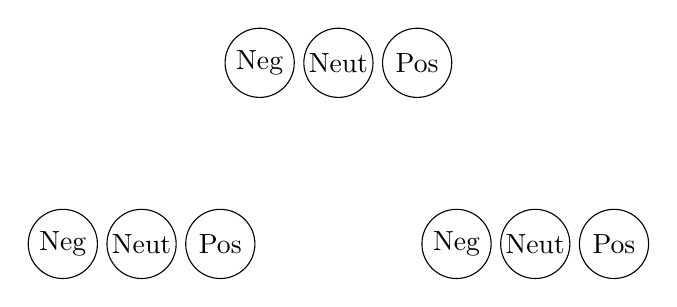
\begin{tikzpicture}
\tikzstyle{xnode}=[rectangle,draw,fill=gray76,align=center,minimum size=2em,text width=2.2em] %
\tikzstyle{lnode}=[circle,draw,fill=white,inner sep=1pt,minimum size=2.5em] %
\tikzstyle{ynode}=[circle,draw,fill=gray76,inner sep=1pt,minimum size=2.5em] %
\tikzstyle{label}=[] %
\tikzstyle{extext}=[] %
\tikzstyle{factor}=[rectangle,fill=black,midway,inner sep=0pt,minimum size=0.4em] %

\node[lnode] (1Neg) at (5 , 3.7) {Neg};
\node[lnode] (1Neut) at (6, 3.7) {Neut};
\node[lnode] (1Pos) at (7, 3.7) {Pos};
\hyperNode{1Neg}{1Neut}{1Pos}{EDU 1};
\crfFeatures{0/5/0.007, 1/6/0.985, 2/7/0.007}{1}{2.4};

\node[lnode] (2Neg) at (2.5, 1.4) {Neg};
\node[lnode] (2Neut) at (3.5, 1.4) {Neut};
\node[lnode] (2Pos) at (4.5, 1.4) {Pos};
\hyperNode{2Neg}{2Neut}{2Pos}{EDU 2};
\crfEdgesLatent{1}{2};
\crfFeatures{0/2.5/0.001, 1/3.5/0.998, 2/4.5/0.001}{2}{0.1};

\node[lnode] (3Neg) at (7.5, 1.4) {Neg};
\node[lnode] (3Neut) at (8.5, 1.4) {Neut};
\node[lnode] (3Pos) at (9.5, 1.4) {Pos};
\hyperNode{3Neg}{3Neut}{3Pos}{EDU 3};
\crfEdgesLatent{1}{3};
\crfFeatures{0/7.5/1., 1/8.5/0., 2/9.5/0.}{3}{0.1};
\end{tikzpicture}
}
%% {
%%   "toks": [
%%     {
%%       "form": "Die",
%%       "prnt": 1,
%%       "lemma": "die",
%%       "tag": "ART",
%%       "rel": "NK",
%%       "children": [],
%%       "feats": {
%%         "case": "nom",
%%         "mmax": {},
%%         "number": "pl",
%%         "UNKFEAT": "*"
%%       }
%%     },
%%     {
%%       "form": "NSA",
%%       "prnt": 2,
%%       "lemma": "nsa",
%%       "tag": "NE",
%%       "rel": "SB",
%%       "children": [
%%         0
%%       ],
%%       "feats": {
%%         "case": "nom",
%%         "mmax": {},
%%         "number": "pl",
%%         "UNKFEAT": "*"
%%       }
%%     },
%%     {
%%       "form": "weiss",
%%       "prnt": -1,
%%       "lemma": "wissen",
%%       "tag": "VVFIN",
%%       "rel": "_",
%%       "children": [
%%         1,
%%         4
%%       ],
%%       "feats": {
%%         "person": "3",
%%         "UNKFEAT": "ind",
%%         "number": "sg",
%%         "mmax": {}
%%       }
%%     },
%%     {
%%       "form": "auch",
%%       "prnt": 4,
%%       "lemma": "auch",
%%       "tag": "ADV",
%%       "rel": "MO",
%%       "children": [],
%%       "feats": {
%%         "mmax": {}
%%       }
%%     },
%%     {
%%       "form": "von",
%%       "prnt": 2,
%%       "lemma": "von",
%%       "tag": "APPR",
%%       "rel": "OP",
%%       "children": [
%%         3,
%%         5
%%       ],
%%       "feats": {
%%         "mmax": {}
%%       }
%%     },
%%     {
%%       "form": "dir",
%%       "prnt": 4,
%%       "lemma": "du",
%%       "tag": "PRF",
%%       "rel": "NK",
%%       "children": [
%%         6
%%       ],
%%       "feats": {
%%         "mmax": {}
%%       }
%%     },
%%     {
%%       "form": "...",
%%       "prnt": 5,
%%       "lemma": "...",
%%       "tag": "$.",
%%       "rel": "--",
%%       "children": [],
%%       "feats": {
%%         "mmax": {}
%%       }
%%     },
%%     {
%%       "form": "Nützt",
%%       "prnt": -1,
%%       "lemma": "nützen",
%%       "tag": "VVFIN",
%%       "rel": "_",
%%       "children": [
%%         8,
%%         9,
%%         10
%%       ],
%%       "feats": {
%%         "person": "3",
%%         "UNKFEAT": "ind",
%%         "tense": "pres",
%%         "number": "sg",
%%         "mmax": {}
%%       }
%%     },
%%     {
%%       "form": "uns",
%%       "prnt": 7,
%%       "lemma": "wir",
%%       "tag": "PPER",
%%       "rel": "OA",
%%       "children": [],
%%       "feats": {
%%         "case": "acc",
%%         "mmax": {},
%%         "person": "1",
%%         "number": "pl",
%%         "UNKFEAT": "*"
%%       }
%%     },
%%     {
%%       "form": "auch",
%%       "prnt": 7,
%%       "lemma": "auch",
%%       "tag": "ADV",
%%       "rel": "MO",
%%       "children": [],
%%       "feats": {
%%         "mmax": {}
%%       }
%%     },
%%     {
%%       "form": "nichts",
%%       "prnt": 7,
%%       "lemma": "nichts",
%%       "tag": "PIS",
%%       "rel": "OA",
%%       "children": [
%%         11
%%       ],
%%       "feats": {
%%         "mmax": {},
%%         "UNKFEAT": "neut"
%%       }
%%     },
%%     {
%%       "form": ".",
%%       "prnt": 10,
%%       "lemma": ".",
%%       "tag": "$.",
%%       "rel": "--",
%%       "children": [],
%%       "feats": {
%%         "mmax": {}
%%       }
%%     },
%%     {
%%       "form": "%NegSmiley",
%%       "prnt": -1,
%%       "lemma": "%negsmiley",
%%       "tag": "ITJ",
%%       "rel": "_",
%%       "children": [],
%%       "feats": {
%%         "mmax": {}
%%       }
%%     }
%%   ],
%%   "msg_id": "394835836069773312",
%%   "text": "Die NSA weiss auch von dir ... Nützt uns auch nichts . %NegSmiley",
%%   "edus": [
%%     {
%%       "polarity_scores": [
%%         0.0066467877477407455,
%%         0.9854232668876648,
%%         0.007929954677820206
%%       ],
%%       "type": "HS",
%%       "prnt_edu": null,
%%       "toks": [
%%         0,
%%         1,
%%         2,
%%         3,
%%         4,
%%         5,
%%         6
%%       ]
%%     },
%%     {
%%       "polarity_scores": [
%%         0.0011337995529174805,
%%         0.9977869391441345,
%%         0.0010792326647788286
%%       ],
%%       "type": "HS",
%%       "prnt_edu": null,
%%       "toks": [
%%         7,
%%         8,
%%         9,
%%         10,
%%         11
%%       ]
%%     },
%%     {
%%       "polarity_scores": [
%%         0.9999760389328003,
%%         1.820568650146015e-05,
%%         5.775107183580985e-06
%%       ],
%%       "type": "FRE",
%%       "prnt_edu": null,
%%       "toks": [
%%         12
%%       ]
%%     }
%%   ],
%%   "rst_trees": {
%%     "chenlo": {
%%       "rel2par": null,
%%       "n/s": null,
%%       "children": [
%%         {
%%           "rel2par": "background",
%%           "n/s": "Satellite",
%%           "children": [],
%%           "id": 0
%%         },
%%         {
%%           "rel2par": "span",
%%           "n/s": "Nucleus",
%%           "children": [
%%             {
%%               "rel2par": "background",
%%               "n/s": "Satellite",
%%               "children": [],
%%               "id": 1
%%             },
%%             {
%%               "rel2par": "span",
%%               "n/s": "Nucleus",
%%               "children": [],
%%               "id": 2
%%             }
%%           ],
%%           "id": -2
%%         }
%%       ],
%%       "id": -1
%%     },
%%     "heerschop": {
%%       "rel2par": null,
%%       "n/s": null,
%%       "id": -1,
%%       "children": [
%%         {
%%           "rel2par": "background",
%%           "n/s": "Satellite",
%%           "id": 0,
%%           "children": []
%%         },
%%         {
%%           "rel2par": "span",
%%           "n/s": "Nucleus",
%%           "id": -2,
%%           "children": [
%%             {
%%               "rel2par": "background",
%%               "n/s": "Satellite",
%%               "id": 1,
%%               "children": []
%%             },
%%             {
%%               "rel2par": "span",
%%               "n/s": "Nucleus",
%%               "id": 2,
%%               "children": []
%%             }
%%           ]
%%         }
%%       ]
%%     },
%%     "bhatia": {
%%       "id": -1,
%%       "rel2par": null,
%%       "children": [
%%         {
%%           "id": 0,
%%           "rel2par": "non-contrastive",
%%           "children": [],
%%           "n/s": "Nucleus"
%%         },
%%         {
%%           "id": -2,
%%           "rel2par": "non-contrastive",
%%           "children": [
%%             {
%%               "id": 1,
%%               "rel2par": "span",
%%               "children": [],
%%               "n/s": "Nucleus"
%%             },
%%             {
%%               "id": 2,
%%               "rel2par": "non-contrastive",
%%               "children": [],
%%               "n/s": "Satellite"
%%             }
%%           ],
%%           "n/s": "Nucleus"
%%         }
%%       ],
%%       "n/s": null
%%     },
%%     "zhou": {
%%       "rel2par": null,
%%       "children": [
%%         {
%%           "rel2par": "other",
%%           "children": [],
%%           "id": 0,
%%           "n/s": "Nucleus"
%%         },
%%         {
%%           "rel2par": "other",
%%           "children": [
%%             {
%%               "rel2par": "span",
%%               "children": [],
%%               "id": 1,
%%               "n/s": "Nucleus"
%%             },
%%             {
%%               "rel2par": "other",
%%               "children": [],
%%               "id": 2,
%%               "n/s": "Satellite"
%%             }
%%           ],
%%           "id": -2,
%%           "n/s": "Nucleus"
%%         }
%%       ],
%%       "id": -1,
%%       "n/s": null
%%     },
%%     "pcc": {
%%       "id": -1,
%%       "rel2par": null,
%%       "children": [
%%         {
%%           "id": 0,
%%           "rel2par": "background",
%%           "children": [],
%%           "n/s": "Satellite"
%%         },
%%         {
%%           "id": -2,
%%           "rel2par": "span",
%%           "children": [
%%             {
%%               "id": 1,
%%               "rel2par": "background",
%%               "children": [],
%%               "n/s": "Satellite"
%%             },
%%             {
%%               "id": 2,
%%               "rel2par": "span",
%%               "children": [],
%%               "n/s": "Nucleus"
%%             }
%%           ],
%%           "n/s": "Nucleus"
%%         }
%%       ],
%%       "n/s": null
%%     }
%%   },
%%   "label": "negative",
%%   "polarity_scores": [
%%     0.998874843120575,
%%     0.0009919496951624751,
%%     0.00013318551646079868
%%   ]
%% }

      \end{center}
    }
\end{example}

Finally, the last example (\ref{snt:dasa:exmp:last-error}) shows an
error made by the \textsc{Last} baseline system, which predicts the
neutral label for a negative tweet based on the polarity of its
right-most discourse unit.  This unit indeed admits some positive
moments with regard to the sad news expressed in the first segment;
but in contrast to the movie description from
Example~\ref{disc-snt:exmp-pang02}, where the last sentence completely
overturned the polarity of the whole text, this time, the final
opinion does not alter the general negative mood of the tweet, but
merely dampens its effect.
\begin{example}[Error Made by the \textsc{Last} System]\label{snt:dasa:exmp:last-error}
  \noindent\textup{\bfseries\textcolor{darkred}{Tweet:}} {\upshape
    $[$' ( :'( :'( Die letzte Aussprache war wohl das schwerste
      Telefonat meines gesamten Lebens :'( :'( :'($]_1$ $[$Aber wir
      gehen friedlich und als F $\ldots]_2$}\\
  \noindent $[$' ( :'( :'( The last talk was probably the most
    difficult call in my entire life :'( :'( :'($]_1$ $[$But we go
    apart peacefully and as f $\ldots]_1$\\[\exampleSep]
  \noindent\textup{\bfseries\textcolor{darkred}{Gold Label:}}\hspace*{4.3em}\textbf{%
    \upshape\textcolor{midnightblue}{negative}}\\
  \noindent\textup{\bfseries\textcolor{darkred}{Predicted Label:}}\hspace*{2em}\textbf{%
    \upshape\textcolor{black}{neutral*}}
\end{example}

\section{Evaluation}

\subsection{Base Classifier}

The first important aspect, which forms the basis of every DASA method
(but at the same time is also limiting its performance), is the
quality of the base sentiment classifier which predicts the scores for
single EDUs of an RST tree.  To see whether a lexion- or
machine-learning--based CGSA system would be a better starting point
for discourse-aware sentiment inference, we reran our experiments,
replacing the probabilities returned by the LBA system with the scores
returned by the lexicon-based metho of \citet{Hu:04} and the ML
approach of~\citet{Mohammad:13}.  The results of this evaluation are
presented in Figures~\ref{dasa:fig:potts-base-classifier} and
\ref{dasa:fig:sb10k-base-classifier}.

\begin{figure*}[htb]
{ \centering
\begin{subfigure}{\textwidth}
  \centering
  \includegraphics[width=\linewidth]{img/dasa-potts-bc-macro-F1.png}
  \caption{\texttt{Macro-\F{}}}\label{dasa:fig:potts-base-classifier-macro-F1}
\end{subfigure}\\
\begin{subfigure}{\textwidth}
  \centering
  \includegraphics[width=\linewidth]{img/dasa-potts-bc-micro-F1.png}
  \caption{\texttt{Micro-\F{}}}\label{dasa:fig:potts-base-classifier-micro-F1}
\end{subfigure}
}
\caption[PotTS results of discourse-aware classifiers with different
  base classifiers]{Results of discourse-aware sentiment analysis
  methods with different base classifiers on the PotTS
  corpus}\label{dasa:fig:potts-base-classifier}
\end{figure*}

From these figures we can see that the lexicon-based attention
approach is in fact more effective than any alternative coarse-grained
sentiment method for almost all discourse-aware approaches.  A few
exceptions to this general tendency are the macro-\F{} of the
\textsc{Last} system, which surprisingly improves in combination with
the lexicon-based \citeauthor{Hu:04} system, and the micro-averaged
\F{}-score of the \textsc{RDP} and \textsc{Last} solutions, which
attain their best ranks together with the \citeauthor{Mohammad:13}'s
classifier (0.713 and 0.582 respectively).

\begin{figure*}[htb]
{ \centering
\begin{subfigure}{\textwidth}
  \centering
  \includegraphics[width=\linewidth]{img/dasa-sb10k-bc-macro-F1.png}
  \caption{\texttt{Macro-\F{}}}\label{dasa:fig:sb10k-base-classifier-macro-F1}
\end{subfigure}\\
\begin{subfigure}{\textwidth}
  \centering
  \includegraphics[width=\linewidth]{img/dasa-sb10k-bc-micro-F1.png}
  \caption{\texttt{Micro-\F{}}}\label{dasa:fig:sb10k-base-classifier-micro-F1}
\end{subfigure}
}
\caption[SB10k results of discourse-aware classifiers with different
  base classifiers]{Results of discourse-aware sentiment analysis
  methods with different base classifiers on the SB10k
  corpus}\label{dasa:fig:sb10k-base-classifier}
\end{figure*}

This situation, however, looks differently on the SB10k dataset, where
LBA leads to higher macro-scores for the \textsc{DDR}, \textsc{R2N2},
\textsc{WNG}, \textsc{Last}, and \textsc{Root} systems, but the
ML-based approach of \citeauthor{Mohammad:13} improves the results of
the \textsc{LCRF}, \textsc{LMCRF}, \textsc{RDP}, and
\textsc{No-Discourse} methods.  The ML-classifier is also the
unequivocal leader in terms of the micro-averaged \F, yielding the
highest scores for all systems except for the approach of
\citet{Wang:13}.  Unfortunately, the lexicon-based slution of
\citet{Hu:04} performs much weaker in comparison with the other two
systems, with the hgighest macro- and micro-averaged \F{}-scores
running up to 0.422 (\textsc{RDP}) and 0.625 (\textsc{Last})
respectively.  The most disappointing result for us, however, is that
the LMCRF system fails to predict any polar class except for
\textsc{Neutral} when trained on the scores produced by this
classifier.  Likewise, LCRF can hardly beat any other competitor,
reaching merely 0.239 macro\F{}.

\subsection{Parsing Quality and Relation Scheme}

Two other factors that could significantly influence the results of
discourse-aware sentiment systems were the quality of automatic RST
analysis and the set of discourse relations distinguished by the
parsing system.  Although improving the results of the DPLP parser let
alone manually annotating the complete PotTS and SB10k datasets was
beyond the scope of this dissertation, we decided to check whether
using hand-crafted RST trees in the test input could improve the
scores of our tested DASA approaches.  For this purpose, we asked a
student assistant to segment and annotate the discourse structure for
88\% of the PotTS test data\footnote{Unfortunately, we could not
  annotate the whole test set due to time limitations of the student.}
and evaluated all trained systems on these trees.
\begin{table}[htb]
  \begin{center}
    \bgroup \setlength\tabcolsep{0.1\tabcolsep}\scriptsize
    \begin{tabular}{p{0.162\columnwidth} % first columm
        *{9}{>{\centering\arraybackslash}p{0.074\columnwidth}} % next nine columns
        *{2}{>{\centering\arraybackslash}p{0.068\columnwidth}}} % last two columns
      \toprule
      \multirow{2}*{\bfseries Method} & %
      \multicolumn{3}{c}{\bfseries Positive} & %
      \multicolumn{3}{c}{\bfseries Negative} & %
      \multicolumn{3}{c}{\bfseries Neutral} & %
      \multirow{2}{0.068\columnwidth}{\bfseries\centering Macro\newline \F{}} & %
      \multirow{2}{0.068\columnwidth}{\bfseries\centering Micro\newline \F{}}\\
      \cmidrule(lr){2-4}\cmidrule(lr){5-7}\cmidrule(lr){8-10}

      & Precision & Recall & \F{} & %
      Precision & Recall & \F{} & %
      Precision & Recall & \F{} & & \\\midrule

      \multicolumn{12}{c}{\cellcolor{cellcolor}PotTS}\\

      %% General Statistics:
      %% precision    recall  f1-score   support
      %% positive       0.82      0.82      0.82       541
      %% negative       0.66      0.55      0.60       220
      %% neutral       0.69      0.75      0.72       351
      %% avg / total       0.75      0.75      0.75      1112
      %% Macro-Averaged F1-Score (Positive and Negative Classes): 70.96%
      %% Micro-Averaged F1-Score (All Classes): 74.7302%
      LCRF & 0.82 & 0.82 & \textbf{0.82} & %
       \textbf{0.66} & 0.55 & 0.6 & %
       0.69 & 0.75 & 0.72 & %
       0.71 & 0.747\\

      %% General Statistics:
      %% precision    recall  f1-score   support
      %% positive       0.83      0.81      0.82       541
      %% negative       0.65      0.55      0.60       220
      %% neutral       0.69      0.78      0.73       351
      %% avg / total       0.75      0.75      0.75      1112
      %% Macro-Averaged F1-Score (Positive and Negative Classes): 70.86%
      %% Micro-Averaged F1-Score (All Classes): 74.9101%
     LMCRF & \textbf{0.83} & 0.81 & \textbf{0.82} & %
       0.65 & 0.55 & 0.6 & %
       0.69 & \textbf{0.78} & \textbf{0.73} & %
       0.709 & 0.749\\

      %% General Statistics:
      %% precision    recall  f1-score   support
      %% positive       0.80      0.84      0.82       541
      %% negative       0.64      0.58      0.61       220
      %% neutral       0.72      0.71      0.72       351
      %% avg / total       0.75      0.75      0.75      1112
      %% Macro-Averaged F1-Score (Positive and Negative Classes): 71.76%
      %% Micro-Averaged F1-Score (All Classes): 75.0899%
      RDP & 0.8 & 0.84 & \textbf{0.82} & %
       0.64 & 0.58 & 0.61 & %
       \textbf{0.72} & 0.71 & 0.72 & %
       \textbf{0.718} & 0.751\\

      %% General Statistics:
      %% precision    recall  f1-score   support
      %% positive       0.78      0.75      0.77       541
      %% negative       0.58      0.66      0.62       220
      %% neutral       0.66      0.63      0.64       351
      %% avg / total       0.70      0.70      0.70      1112
      %% Macro-Averaged F1-Score (Positive and Negative Classes): 69.31%
      %% Micro-Averaged F1-Score (All Classes): 69.7842%
      DDR & 0.78 & 0.75 & 0.77 & %
       0.58 & \textbf{0.66} & \textbf{0.62} & %
       0.66 & 0.63 & 0.64 & %
       0.693 & 0.698\\

      %% General Statistics:
      %% precision    recall  f1-score   support
      %% positive       0.81      0.82      0.81       541
      %% negative       0.64      0.53      0.58       220
      %% neutral       0.68      0.74      0.71       351
      %% avg / total       0.73      0.74      0.73      1112
      %% Macro-Averaged F1-Score (Positive and Negative Classes): 69.67%
      %% Micro-Averaged F1-Score (All Classes): 73.6511%
      R2N2 & 0.81 & 0.82 & 0.81 & %
       0.64 & 0.53 & 0.58 & %
       0.68 & 0.74 & 0.71 & %
       0.697 & 0.737\\

      %% General Statistics:
      %% precision    recall  f1-score   support
      %% positive       0.58      0.74      0.65       541
      %% negative       0.63      0.19      0.29       220
      %% neutral       0.51      0.51      0.51       351
      %% avg / total       0.56      0.56      0.53      1112
      %% Macro-Averaged F1-Score (Positive and Negative Classes): 46.97%
      %% Micro-Averaged F1-Score (All Classes): 55.7554%
      WNG & 0.58 & 0.74 & 0.65 & %
       0.63 & 0.19 & 0.29 & %
       0.51 & 0.51 & 0.51 & %
       0.47 & 0.558\\

      %% General Statistics:
      %% precision    recall  f1-score   support
      %% positive       0.55      0.86      0.67       541
      %% negative       0.51      0.11      0.18       220
      %% neutral       0.56      0.35      0.43       351
      %% avg / total       0.54      0.55      0.50      1112
      %% Macro-Averaged F1-Score (Positive and Negative Classes): 42.59%
      %% Micro-Averaged F1-Score (All Classes): 55.0360%
      \textsc{Last} & 0.55 & \textbf{0.86} & 0.67 & %
       0.51 & 0.11 & 0.18 & %
       0.56 & 0.35 & 0.43 & %
       0.426 & 0.55\\

      %% General Statistics:
      %% precision    recall  f1-score   support
      %% positive       0.58      0.56      0.57       541
      %% negative       0.58      0.25      0.35       220
      %% neutral       0.43      0.60      0.50       351
      %% avg / total       0.53      0.51      0.50      1112
      %% Macro-Averaged F1-Score (Positive and Negative Classes): 46.03%
      %% Micro-Averaged F1-Score (All Classes): 51.2590%
      \textsc{Root} & 0.58 & 0.56 & 0.57 & %
       0.58 & 0.25 & 0.35 & %
       0.43 & 0.6 & 0.5 & %
       0.46 & 0.513\\

      %% General Statistics:
      %% precision    recall  f1-score   support
      %% positive       0.81      0.84      0.82       541
      %% negative       0.65      0.57      0.61       220
      %% neutral       0.72      0.73      0.73       351
      %% avg / total       0.75      0.75      0.75      1112
      %% Macro-Averaged F1-Score (Positive and Negative Classes): 71.63%
      %% Micro-Averaged F1-Score (All Classes): 75.2698%
      \textsc{No-Discourse} & 0.81 & 0.84 & \textbf{0.82} & %
       0.65 & 0.57 & 0.61 & %
       \textbf{0.72} & 0.73 & \textbf{0.73} & %
       0.716 & \textbf{0.753}\\\bottomrule
    \end{tabular}
    \egroup
    \caption[Results of DASA methods on manually annotated RST
      trees]{Results of discourse-aware sentiment analysis methods on
      the PotTS corpus with manually annotated RST trees}
    \label{dasa:tbl:res-gold}
  \end{center}
\end{table}
As we can see from the results in Table~\ref{dasa:tbl:res-gold}, the
scores of all systems except \textsc{WNG}, \textsc{Last}, and
\textsc{Root} increase by three to four percent.  Even the macro- and
micro-averaged \F{}-measures of the discourse-unaware classifier raise
from 0.677 and 0.706 to 0.716 and 0.753 respectively.  This latter
change, however, is exclusively due to the reduced size of the test
set and not the improved discourse structure of the input.  This time,
the discourse-unware method also surpasses all other competitors in
terms of the micro-averaged \F{}, achieving an accuracy of 75,3\%, but
still fails to outperform the Recursive Dirichlet Process on the
macro-averaged metric, getting a 0.2\% worse score than RDP (0.716
versus 0.718 macro-\F{}).  Despite its signifcant improvements, the
LMCRF method cannot surpass the plain LBA classifier, although it gets
the same \F{}-scores for the positive and neutral classes as the
discourse-unaware method.  The most unexpected finding for us though
is that in gold discourse structures (as annotated by our student),
EDUs which control the actual polarity of the message are unlikely to
appear at the extreme ends of these structures either in horizontal
(as the last segment of the message) or in vertical order (as the root
of the discourse tree), which leads to a degradation of the scores for
the \textsc{Last} and \textsc{Root} methods.

As you might remember from the beginning of this chapter, while
preparing the data for our experiments, we decided to only
differentiate between \textsc{Contrastive} and
\textsc{Non-Contrastive} links, drawing on a similar idea by
\citet{Bhatia:15}.  The main reason for this simplification was to
ease the work of the RST parser and DASA methods by decreasing the
number of their distinguished classes and consequently reducing the
number of learned parameters.  Although similar approximations were
made in almost all other works on discourse-aware opinion mining
\cite[see ][]{Chenlo:13,Heerschop:11,Zhou:11}, it was unclear to us
whether this subset of relations was indeed optimal and sufficient to
reflect all possible varieties of discourse interactions that could
exist in text and play a role in sentiment composition.

To investigate this question in more detail, we decided to repeat our
experiments, using the subsets of relations proposed by
\citet{Chenlo:13}, \citet{Heerschop:11}, and \citet{Zhou:11}, and also
try the original full set of all discourse links from the Potsdam
Commentary Corpus.  A detailed overview of these relation schemes is
shown in Table~\ref{dasa:tbl:rst-rel-sets}.

\begin{table}[h]
  \begin{center}
    \bgroup
    \setlength\tabcolsep{0.3\tabcolsep}\scriptsize
    \begin{tabular}{p{0.17\columnwidth} % first columm
        *{1}{>{\centering\arraybackslash}p{0.4\columnwidth}}
        *{1}{>{}p{0.4\columnwidth}}} % next two columns
      \toprule
      \textbf{Scheme} & \textbf{Relation Set} & {\centering\textbf{Equivalence Classes}}\\\midrule

      \citeauthor{Bhatia:15} & \{\textsc{Contrastive},
      \textsc{\bfseries Non-Contrastive}\} & \textsc{Contrastive} $\defeq$
      \{\textsc{Antithesis}, \textsc{Antithesis-E},
      \textsc{Comparison}, \textsc{Concession},
      \textsc{Consequence-S}, \textsc{Contrast},
      \textsc{Problem-Solution}\}.\\

      \citeauthor{Chenlo:13} & \{\textsc{Attribution},
      \textsc{Background}, \textsc{Cause}, \textsc{Comparison},
      \textsc{Condition}, \textsc{Consequence}, \textsc{Contrast},
      \textsc{Elaboration}, \textsc{Enablement}, \textsc{Evaluation},
      \textsc{Explanation}, \textsc{Joint}, \textsc{Otherwise},
      \textsc{Temporal}, \textsc{\bfseries Other}\} & \\

      \citeauthor{Heerschop:11} & \{\textsc{Attribution},
      \textsc{Background}, \textsc{Cause}, \textsc{Condition},
      \textsc{Contrast}, \textsc{Elaboration}, \textsc{Enablement},
      \textsc{Explanation}, \textsc{\bfseries Other}\} & \\

      \textsc{PCC} & \{\textsc{Antithesis}, \textsc{Background},
      \textsc{Cause}, \textsc{Circumstance}, \textsc{Concession},
      \textsc{Condition}, \textsc{Conjunction}, \textsc{Contrast},
      \textsc{Disjunction}, \textsc{E-Elaboration},
      \textsc{Elaboration}, \textsc{Enablement},
      \textsc{Evaluation-N}, \textsc{Evaluation-S}, \textsc{Evidence},
      \textsc{Interpretation}, \textsc{Joint}, \textsc{Justify},
      \textsc{List}, \textsc{Means}, \textsc{Motivation},
      \textsc{Otherwise}, \textsc{Preparation}, \textsc{Purpose},
      \textsc{Reason}, \textsc{Restatement}, \textsc{Restatement-MN},
      \textsc{Result}, \textsc{Sequence}, \textsc{Solutionhood},
      \textsc{Summary}, \textsc{Unconditional}, \textsc{Unless},
      \textsc{Unstated-Relation}\} & \\

      \citeauthor{Zhou:11} & \{\textsc{Contrast}, \textsc{Condition},
      \textsc{Continuation}, \textsc{Cause}, \textsc{Purpose},
      \textsc{\bfseries Other}\} & \textsc{Contrast} $\defeq$
      \{\textsc{Antithesis}, \textsc{Concession}, \textsc{Contrast},
      \textsc{Otherwise}\};\newline \textsc{Continuation} $\defeq$
      \{\textsc{Continuation}, \textsc{Parallel}\};\newline
      \textsc{Cause} $\defeq$ \{\textsc{Evidence}, \textsc{Nonvolitional-Cause},
      \textsc{Nonvolitional-Result}, \textsc{Volitional Cause},
      \textsc{Volitional-Result}\};\\\bottomrule

    \end{tabular}
    \egroup
    \caption[RST relations used in different discourse-aware sentiment
      methods]{RST relations used in the original Potsdam Commentary
      Corpus and different discourse-aware sentiment methods\\ {\small
        (default relation [which subsumes the rest of the links] is
        highlighted in \textbf{boldface})}}
    \label{dasa:tbl:rst-rel-sets}
  \end{center}
\end{table}

As we can see from the table, our initially chosen scheme is by far
the smallest one, comprising only two elements (\textsc{Contrastive}
and \textsc{Non-Contrastive}), whereas PCC---the most comprehensive
scheme in this study---features a total of 34 links.  In this respect,
other approaches rather steer a middle course, swaying between 6 to 15
relations.

To estimate the utility of these sets, we retrained the DPLP parser
using each of these relation sets. In order to estimate how much the
number of distinguished discourse relations affected the quality of
automatic parsing, we additionally evaluated every newly trained
system on the held-out PCC test data and present their results in
Table~\ref{dasa:tbl:dplp-results}.

\begin{table}[h]
  \begin{center}
    \bgroup \setlength\tabcolsep{0.1\tabcolsep}\scriptsize
    \begin{tabular}{p{0.22\columnwidth} % first columm
        *{3}{>{\centering\arraybackslash}p{0.25\columnwidth}}} \toprule

      \textbf{Relation Scheme} & \textbf{Span \F{}} &
      \textbf{Nuclearity \F{}} & \textbf{Relation \F{}}\\\midrule

      \citet{Bhatia:15} & \textbf{0.777} & 0.512 & \textbf{0.396}\\

      \citet{Chenlo:13} & 0.769 & 0.505 & 0.362\\

      \citet{Heerschop:11} & 0.774 & 0.51 & 0.361\\

      \textsc{PCC} & 0.776 & \textbf{0.534} & 0.326\\

      \citet{Zhou:11} & 0.776 & 0.501 & 0.388\\\bottomrule
    \end{tabular}
    \egroup
    \caption[Results of RST parser on PCC~2]{Results of automatic RST
      parser on PCC~2.0 with different relation schemes}
    \label{dasa:tbl:dplp-results}
  \end{center}
\end{table}

As is evident from the scores, a coarser relation scheme might indeed
lead to better parsing quality, especially in terms of relation \F{}.
In the most extreme cases (\eg{} \citeauthor{Bhatia:15} versus PCC),
these gains can even run up to seven percent. However, with respect to
other metrics (first of all, span and nuclearity \F{}), these gaps are
not that big and in some cases might even be in favor of the richer
set (\eg{} nuclearity \F{} for PCC).

To see how this varying quality could affect the net results of
discourse-aware sentiment methods, we re-evaluated all DASA approaches
on the updated automatic RST trees and present the results of this
evaluation in Figure~\ref{dasa:fig:potts-rel-schemes}.

\begin{figure*}[htb]
{
\centering
\begin{subfigure}{\textwidth}
  \centering
  \includegraphics[width=\linewidth]{img/dasa-potts-macro-F1.png}
  \caption{\texttt{Macro-\F{}}}\label{dasa:fig:potts-rel-schemes-macro-F1}
\end{subfigure}\\
\begin{subfigure}{\textwidth}
  \centering
  \includegraphics[width=\linewidth]{img/dasa-potts-micro-F1.png}
  \caption{\texttt{Micro-\F{}}}\label{dasa:fig:potts-rel-schemes-micro-F1}
\end{subfigure}
}
\caption[PotTS results of discourse-aware classifiers with different
  relation schemes]{Results of discourse-aware sentiment classifiers
  for different relation schemes on the PotTS
  corpus}\label{dasa:fig:potts-rel-schemes}
\end{figure*}

As it turns out, latent marginalized CRF can still hold the overall
record in terms of both macro- and micro-averaged \F{} on the PotTS
corpus, although its margin to the closest competitor (R2N2) is
relatively small this time, reducing to only 0.1 percent.
Interestingly enough, both top-performing methods (LMCRF and R2N2)
achieve their best results with richer relation schemes than the one
we used in our initial experiment: For example, LMCRF attains its
highest macro-score when used with the relation set defined
by~\citet{Heerschop:11} and yields the best micro-\F{} with the scheme
by~\citet{Chenlo:14}.  The rhetorical recusrive neural network, vice
versa, attains its highest macro-average with the latter relation set
and reaches its best micro-score when used with the discourse links
proposed by~\citeauthor{Heerschop:11}.

A different situation is observed with other approaches though: For
example, latent CRF and Recursive Dirichlet Process perform best when
used with the initial smallest set by \citet{Bhatia:15}.  On the other
hand, discourse-depth reweighting strongly benefits from the full
unconstrained PCC set, which might be partially due to the better
nuclearity prediction achieved with this scheme.  Finally, the
\textsc{WNG} and \textsc{Root} methods get their best results with the
subsets proposed by~\citet{Chenlo:14} and \citet{Heerschop:11}
respectively.

\begin{figure*}[htb]
{ \centering
\begin{subfigure}{\textwidth}
  \centering
  \includegraphics[width=\linewidth]{img/dasa-sb10k-macro-F1.png}
  \caption{\texttt{Macro-\F{}}}\label{dasa:fig:sb10k-rel-schemes-macro-F1}
\end{subfigure}\\
\begin{subfigure}{\textwidth}
  \centering
  \includegraphics[width=\linewidth]{img/dasa-sb10k-micro-F1.png}
  \caption{\texttt{Micro-\F{}}}\label{dasa:fig:sb10k-rel-schemes-micro-F1}
\end{subfigure}
}
\caption[SB10k results of discourse-aware classifiers for different
  relation schemes]{Results of discourse-aware sentiment classifiers
  for different relation schemes on the SB10k
  corpus}\label{dasa:fig:sb10k-rel-schemes}
\end{figure*}

As we can see from Figure~\ref{dasa:fig:sb10k-rel-schemes}, the
performance of our methods is much more uniform on the SB10k corpus,
where their \F-scores vary only slightly across the different relation
schemes.  The only significant improvement that we can notice this
time is higher macro- and micro-average achieved by the RDP approach
in conjunction with the \citeauthor{Heerschop:11}'s relation set.
Somewhat surprisingly, this set is also most amenable to the
\textsc{Root} method, which reaches 0.488 macro-\F{} and 0.663
micro-\F{} with this set, significantly improving on its initial
benchmark.  On the other hand, discourse-depth reweighting and the
approach by~\citet{Wang:13} benefit from the relations used
by~\citet{Chenlo:13} so much that the former system even achieves the
highest overall macro-score (0.572) on this dataset, being on a par
with the R2N2 system, which reaches its best results with the
\citeauthor{Zhou:11}'s set (0.572 macro-\F{} and 0.719 micro-\F{}).

\section{Summary and Conclusions}

Summarizing our findings, we would like to recap that in this chapter
we have made the following contributions and discovered the following
facts:
\begin{itemize}
  \item first if all, we have presented a comprehensive overview of
    the most popular approaches to automatic discourse analysis that
    exist in the literature nowadays and explained why one of these
    frameworks (Rhetorical Structure Theory) would be a more
    appropriate basis for enhancing a sentiment analysis system with
    discourse information than the others;
  \item to check whether our lexicon-based attention system from the
    previous chapter would indeed achieve better scores when working
    on the RST tree of a tweet than when analyzing it as a whole at
    once, disregarding of its discourse structure, we have segmented
    all microblogs from the PotTS and SB10k corpora with an SVM-based
    discourse segmenter~\cite{Sidarenka:15}, getting 4,771 and 3,763
    multi-EDU microblogs respectively;
  \item in order to obtain discourse trees for the above tweets, we
    have retrained one of the recent state-of-the-art English RST
    parsers \cite[DPLP; ][]{Ji:14} on the German Potsdam Commentary
    Corpus~\cite{Stede:14} and applied it to the aforementioned PotTS
    and SB10k messages;
  \item to estimate the results of the existing discourse-aware
    sentiment analysis systems, we have reimplemented the DASA
    approaches of~\citet{Wang:15} and \citet{Bhatia:15} and also
    established two simpler baselines, in which we predicted the
    semantic orientation of a tweet based on the polarity of its root
    and last EDUs, and evaluated these methods on the automatically
    parsed data, getting the best results with the R2N2 solution
    of~\citet{Bhatia:15} (0.657 and 0.559 macro-\F{} on PotTS and
    SB10k respectively);
  \item we could, however, further improve these results with our
    three proposed novel solutions: latent and latent marginalized
    conditional random fields and recursive Dirichlet process,
    boosting the macro-averaged \F{}-scores to 0.678 on PotTS and
    0.56\F{} on SB10k;
  \item an evaluation of these methods with different settings showed
    that these scores largely correlated with the results of the base
    sentiment classifier (the one we used to predict the polarity of a
    single EDU) and also revealed an important drawback of the latent
    marginalized CRF system, which failed to predict any negative
    instance on the test set of the PotTS corpus when used in
    conjunction with the lexicon-based approach of~\citet{Hu:04};
  \item nevertheless, almost all DASA approaches except for the most
    simple ones could get better scores than in our initial
    experiments when operating on manually annotated RST trees or
    using a richer relation scheme than the one proposed
    by~\citet{Bhatia:15};
  \item finally, we could show that discourse-aware methods could
    outperform the plain lexicon-based attention system in almost all
    settings (the only exception was the micro-averaged \F{}-score on
    the manually annotated PotTS trees), although the margin of these
    improvements was moderate.  We can, however, imagine that ths
    margin might further increase if we apply discourse-aware methods
    to messages of greater text length or take the whole discussion
    thread into account.
\end{itemize}
